\chapter{Operazioni e strutture algebriche}
\section{Generalità sulle operazioni}

\begin{defbox}{Operazioni binarie}\index{Operazione!Binaria}
	Se $S$ è un insieme non vuoto, un'applicazione
	\begin{displaymath}
		\bot: S \times S \longrightarrow S
	\end{displaymath}
	si chiama \textbf{operazione binaria} (ovunque definita) in $S$. Qualunque siano gli elementi $x$ e $y$ di $S$,	l'immagine $\bot(x,y)$ della coppia $x,y$ mediante $\bot$ si dice \textbf{composto} di $x$ e $y$, e si denota col simbolo $x \bot y$.
\end{defbox}

\begin{example}
	\begin{enumerate}
		\item In $\mathbb{Z}$ sono operazioni binarie le operazioni di addizione, sottrazione e moltiplicazione.
	
		\item La divisione non è un'operazione binaria in $\mathbb{Z}$ in quanto non tutte le coppie $(m,n) \in \mathbb{Z}^{2}$ godono di composto. Ad esempio $(2,4)$, infatti: $2 \divslash 4 \notin \mathbb{Z}$.
	
		\item Fissato un insieme $A$ è possibile considerare l'insieme delle parti $\mathcal{P}(A)$. In $\mathcal{P}(A)$ è possibile considerare come operazioni binarie tutte le operazioni di intersezione, unione, differenza simmetrica e differenza, ecc.
	\end{enumerate}
\end{example}

Esiste un modo per rappresentare in tabella un'operazione. Supponiamo che l'insieme $S$ sia composto da tre elementi: $$S =\{a,b,c\}$$ Consideriamo un'operazione $\bot : S \times S \rightarrow S$ che può essere rappresentata mediante una tabella come mostrato qui di seguito:
\begin{center}
	\begin{tblr}{hlines,vlines,row{1}={primary!40!white},column{1}={primary!40!white},cells={mode=math},colspec={cccc}}
		\bot & a & b & c \\
		a & a \bot a & a \bot b & a \bot c \\
		b & b \bot a & b \bot b & b \bot c \\
		c & c \bot a & c \bot b & c \bot c \\
	\end{tblr}
\end{center}

Queste tabelle prendono il nome di \textbf{tavole di Cayley}.\index{Cayley}

\subsection{Proprietà delle operazioni}

\begin{defbox}{Operazioni associative}
	Sia $S$ un insieme non vuoto. Un'operazione $\bot: S \times S \longrightarrow S$ si dice \textbf{associativa} se risulta:
	\begin{displaymath}
		\forall x,y,z \in S \bigl( (x \: \bot \: y)\: \bot \: z = x \: \bot \: (y \:  \bot \: z)\bigr)
	\end{displaymath}
\end{defbox}


\begin{example}
	Sono un esempio di operazioni associative tutte le operazioni insiemistiche come l'unione, l'intersezione, la differenza simmetrica, l'unione unaria e l'intersezione unaria.
\end{example}

\begin{defbox}{Operazioni commutative}\index{Commutatività}
	Sia $S$ un insieme non vuoto. Un'operazione $\bot: S \times S \longrightarrow S$ si dice \textbf{commutativa} se risulta:
	\begin{displaymath}
		\forall x,y \in S \bigl(x \: \bot \: y = y \: \bot \: x\bigr)
	\end{displaymath}
	Due elementi $a,b$ di $S$ tali che $a \bot b = b \bot a$ si dicono \textbf{permutabili}.
\end{defbox}


\begin{osservation}
	È possibile determinare la proprietà commutativa di un'operazione osservando la relativa tavola di Cayley. Infatti, un'operazione gode della proprietà commutativa se e solo se la tavola di Cayley è \textit{simmetrica} lungo la propria diagonale.
\end{osservation}


\begin{example}
	Sia $s=\{a,b\}$, è possibile quindi considerare l'insieme $\mathcal{P}(s) = \{ \emptyset, \{a\}, \{b\}, s\}$ e l'operazione binaria interna $\cap : \mathcal{P}(s) \times \mathcal{P}(s) \rightarrow \mathcal{P}(s)$. Come ben sappiamo l'intersezione gode della proprietà commutativa e possiamo ben osservarlo costruendo la tavola di Cayley:
	\begin{center}
		\begin{tblr}
			{
				hlines,
				vlines,
				row{1}={primary!40!white},
				column{1}={primary!40!white},
				cells={mode=math},
				colspec={ccccc}
			}
			\cap & \emptyset & \{a\} & \{b\} & s \\
			\emptyset & \emptyset & \emptyset & \emptyset & \emptyset\\
			\{a\} & \emptyset & \{a\} & \emptyset & \{a\} \\
			\{b\} & \emptyset & \emptyset & \{b\} & \{b\} \\
			s & \emptyset & \{a\} & \{b\} & s
		\end{tblr}
	\end{center}
	\smallskip
	
	Infatti, osservando le celle dello stesso colore osserviamo che la tavola è simmetrica lungo la diagonale secondaria. Notiamo inoltre che, nonostante $\cap$ goda anche della proprietà associativa questa non può essere osservata dalla tavola ed è necessario quindi eseguire un controllo diretto tra tutte le possibili composte.
\end{example}

\begin{example}
	La sottrazione in $\mathbb{Z}$ non gode della proprietà commutativa e associativa. Infatti:
	\begin{displaymath}
		\forall a,b \in \mathbb{Z} \qquad a-b \neq b-a
	\end{displaymath}
	Infatti: $3-2\neq 2-3$.
	Per verificare l'associatività di una operazione è comodo verificare prima se essa gode della proprietà commutativa in quanto questa può velocizzare significativamente i calcoli. La sottrazione è associativa in $\mathbb{Z}$ se e solo se:
	\begin{displaymath}
		\forall a,b,c \in \mathbb{Z} \qquad \bigl( (a-(b-c)) = (a-b)-c \bigr)
	\end{displaymath}
	Per procedere avanti nella dimostrazione si osserva che: $a-(b-c)=(a-b)+c$. Quindi per essere associativa l'operazione deve valere:
	\begin{displaymath}
		(a-b)+c = (a-b)-c
	\end{displaymath}
	ma qualsiasi sia la terna, ad esempio $(0,0,1)$, si ha:
	\begin{displaymath}
		(0-0)+1\neq (0-0)-1
	\end{displaymath}
	Quindi l'operazione non è associativa in $\mathbb{Z}$.
\end{example}

\begin{teorbox}[Teorema di associatività]
	Se un'operazione $\star$ è associativa, presi $n$ elementi, qualsiasi sia l'ordine delle operazioni, il risultato è sempre lo stesso.
\end{teorbox}


\begin{teorbox}[Teorema di commutatività]
	Se un'operazione $\star$ è associativa e commutativa, dati $n$ elementi, qualsiasi sia l'ordine delle operazioni e degli operandi il risultato non cambia.
\end{teorbox}

\begin{example}
	L'associatività e la commutatività \textit{non sono correlate} tra di loro. Prendiamo ad esempio l'operazione binaria in $\mathbb{Z}$ definita come:
	\begin{displaymath}
		\forall a,b \in \mathbb{Z} \qquad a \ast b = (a+b)^{2}
	\end{displaymath}
	Questa operazione è banalmente commutativa in quanto:
	\begin{displaymath}
		\forall a,b \in \mathbb{Z} \qquad a \ast b = (a+b)^{2}=(b+a)^{2}=b \ast a
	\end{displaymath}
	ma non è associativa. Infatti, per essere associativa dovrebbe essere:
	\begin{displaymath}
		\forall a,b,c \in \mathbb{Z} \qquad a \ast (b \ast c) = (a \ast b) \ast c
	\end{displaymath}
	ma $$a \ast (b \ast c) = a \ast (b+c)^{2} = \bigl(a + (b+c)^{2}\bigr)^{2}$$
	e $$(a \ast b) \ast c = c \ast (a \ast b) = \bigl(c + (a+b)^{2}\bigr)^{2} $$
	sono diverse in quanto rappresentano due espressioni diverse qualunque sia la terna $(a,b,c)$.
\end{example}

\begin{defbox}{Operazioni distributive}\index{Distributività}
	Se $\bot$ e $\star$ sono operazioni in S, si dice che $\star$ è \textbf{distributiva a destra} rispetto a $\bot$ se per ogni terna $x,y,z$ di elementi di $S$ risulta
	\begin{equation}
		(x\: \bot \: y)\: \star \: z \;=\;(x \: \star z)\: \bot \: (y \: \star \: z)
	\end{equation}
Sarà \textbf{distributiva a sinistra} rispetto a $\bot$ se per ogni terna $x,y,z \in S$ risulta:
\begin{equation}
	x \ \star \ (y \ \bot \ z) = (x  \ \star \ y) \ \bot \ (x \ \star \ z) 
\end{equation}
Quando $\star$ è commutativa, allora le due condizioni sono equivalenti.
\end{defbox}

\begin{example}
\begin{enumerate}
	\item 	In $\mathbb{N}$ possiamo considerare le operazioni $\cdot$ e $+$ che corrispondono alle operazioni usuali di moltiplicazioni e addizione. Dalle proprietà dell'aritmetica sappiamo che vale la proprietà distributiva della moltiplicazione rispetto all'addizione:
	\begin{displaymath}
		\forall a,b,c \in \mathbb{N} \bigl(a \cdot (b+c) = a \cdot b + a \cdot c \bigr)
	\end{displaymath}
	\item L'unione insiemistica è distributiva rispetto all'intersezione, e l'intersezione è distributiva rispetto all'unione. Inoltre l'intersezione è distributiva rispetto alla differenza simmetrica.
\end{enumerate}
\end{example}

\begin{defbox}{Operazione opposta}\index{Operazione!Opposta}
	Sia $\ast: S \times S \longrightarrow S$ una operazione binaria in $S$. È possibile considerare l'\textbf{operazione opposta}\index{Operazione opposta} $\ast^{\ast}$ definita ponendo:
	\begin{equation}
		\forall a,b \in S (a \ast^{\ast}b=b \ast a)
	\end{equation}
	
\end{defbox}
L'operazione opposta ha le stesse proprietà dell'operazione iniziale. Riferendosi alla rappresentazione grafica delle tavole di Cayley, calcolare l'operazione opposta significa ribaltare la tavola rispetto a righe e colonne. 

\begin{osservation}
	Una operazione è commutativa se e solo se essa coincide con la propria operazione opposta.
\end{osservation}

\section{Strutture algebriche}
\subsection{Semigruppi}\index{Semigruppi}

\begin{defbox}{Struttura algebrica}\index{Struttura algebrica}
	Sia $S$ un insieme non vuoto e siano $\bot_{1},...,\bot_{n}$ $n$ operazioni in S. La $n+1$-pla $(S,\bot_{1},...,\bot_{n})$ si chiama \textbf{struttura algebrica} e l'insieme $S$ si chiama \textbf{sostegno} di tale struttura.
\end{defbox}

\begin{defbox}{Semigruppo}
	Una struttura algebrica ad una operazione interna $(S, \bot)$ si dice \textbf{semigruppo} se l'operazione $\bot$ è associativa. Un semigruppo $(S,\bot)$ si dice \textbf{commutativo} o \textbf{abeliano} se l'operazione $\bot$ è anche commutativa.
\end{defbox}

\begin{example}
\begin{enumerate}
	\item Gli insiemi $\mathbb{N},\mathbb{Z},\mathbb{Q},\mathbb{R}$ con l'usuale operazione somma sono tutti semigruppi. Analogamente se invece della somma consideriamo il prodotto.

	\item Sia $A$ un insieme, sia $A^{A}$ l'insieme delle funzioni $f:A \rightarrow A$ e sia $\circ$ la composizione di funzioni. Possiamo considerare la composizione come un'operazione su $A^{A}$:
	\begin{displaymath}
		\circ : (f,g) \in A^{A} \times A^{A} \mapsto f \circ g \in A^{A}
	\end{displaymath}
	Dato che $\circ$ è associativa la struttura $(A^{A},\circ)$ è un semigruppo.
	\item Consideriamo $\mathbb{Z}$ e la funzione $-: \mathbb{Z} \times \mathbb{Z}: (a,b) \mapsto a-b$. La funzione $-$ è un'operazione, ma non è associativa. Infatti è possibile trovare almeno una terna $a,b,c \in \mathbb{Z}$ per cui $a-(b-c)\neq (a-b)-c$. Per esempio $a=4$, $b=-2$, $c=8$:
	\[(4-(-2))-8=-2 \neq 10=4-(-2-8)\]
	Quindi l'operazione $-$ non dà su $\mathbb{Z}$ la struttura di semigruppo.
	\item Su $\mathbb{R} \times \mathbb{R}$ definiamo $(a,b) \ast (c,d)=(ac,ad+b)$. $(\mathbb{R}\times \mathbb{R},\ast)$ è un semigruppo. Infatti:
	\begin{align*}
		\forall (a,b),(c,d),(e,f) \in \mathbb{R}\times\mathbb{R}\Bigl((a,b)\ast \bigl((c,d) \ast (e,f)\bigr) &= (a,b) \ast (ce,cf+d) \\
		&= (ace, acf+ad+b) \\
		&= (ac,ad+b) \ast (e,f) \\
		&= \bigl((a,b)\ast(c,d)\bigr)\ast (e,f)\Bigr)
	\end{align*}
\end{enumerate}
\end{example}

\begin{defbox}{Parte stabile e operazione indotta}\index{Parte stabile}
	Sia $\bot: S \times S \longrightarrow S$ un'operazione nell'insieme non vuoto S. Una parte non vuota $X$ di $S$ si dice \textbf{stabile} o \textbf{chiusa} rispetto a $\bot$ se per ogni coppia $(x,y)$ di elementi di $X$ anche il composto $x\: \bot \: y$ appartiene a $X$. In questo caso l'applicazione
	\begin{displaymath}
		\bot_{X}\: : \:(x,y)\in X \times X \longmapsto x \: \bot \: y \in X
	\end{displaymath}
	è un'operazione in $X$, che si dice \textbf{indotta} da $\bot$ su $X$.
\end{defbox}

\begin{example}
	Consideriamo la struttura $(\mathbb{Z}, -)$, chiaramente $\mathbb{N} \subseteq \mathbb{Z}$ non è chiusa rispetto alla sottrazione.
\end{example}

\begin{defbox}{Sottostruttura algebrica}\index{Sottostruttura}
	Sia $(S,\bot_{1},...,\bot_{n})$ una struttura algebrica, e sia $X$ una parte non vuota di $S$ che sia stabile rispetto a ciascuna delle operazioni $\bot_{1},...,\bot_{n}$. La struttura algebrica $(X,\bot_{1},...,\bot_{n})$ si dice \textbf{sottostruttura} di $(S,\bot_{1},...,\bot_{n})$.
\end{defbox}

\begin{defbox}{Potenze in un semigruppo}
	Se $(S,\bot)$ è un semigruppo, possiamo definire le \textbf{potenze} di un elemento $a \in S$ mediante l'induzione:
	\begin{equation}
		\begin{cases*}
			a^{n} = a & \mbox{se } n=1 \\
			a^{n+1} = a^{n} \bot a & \mbox{se } n \geq 1
		\end{cases*}
	\end{equation} 
\end{defbox}

\begin{propbox}
	Sia $(S,\bot)$ un semigruppo. Se $a \in S$ e $m,n \in \mathbb{Z}^{+}$, allora:
	\begin{eqnarray}
		a^{n} \bot a^{m} &=& a^{n+m} \\
		(a^{n})^{m} &=& a^{nm}
	\end{eqnarray}
\end{propbox}
\begin{proof}
	Dimostriamo per induzione su $m$ che $a^{n} \bot a^{m} = a^{n+m}$. Se $m=1$, si ha $a^{n} \bot a^{1}=a^{n} \bot a = a^{n+1}$ per come abbiamo definito la potenza. Supponiamo che la proprietà sia vera per un certo $m$, ossia che valga $a^{n}\bot a^{m}= a^{n+m}$, e dimostriamo che allora vale la proprietà anche per l'intero successivo $m+1$, ossia che si ha $a^{n}\bot a^{m+1}=a^{n+m+1}$. Si hanno le uguaglianze:
	\begin{align*}
		a^{n} \bot a^{m+1} &= a^{n} \bot (a^{m}\bot a) & \text{\textcolor{gray}{(Per definizione di potenza)}} \\
		&= (a^{n} \bot a^{m}) \bot a & \text{\textcolor{gray}{(Per l'associatività di $\bot$)}}\\
		&= (a^{n+m}) \bot a & \text{\textcolor{gray}{(Per ipotesi induttiva)}}\\
		&= a^{n+m+1} & \text{\textcolor{gray}{(Per definizione di potenza)}}
	\end{align*}
Dimostriamo ora per induzione su $m$ che $(a^{n})^{m}=a^{nm}$. Per $m=1$, $(a^{n})^{1}=a^{n}=a^{n\cdot1}$. Supponiamo ora che sia vero che $(a^{n})^{m}=a^{nm}$ e otteniamo la catena di uguaglianze:
\begin{align*}
	(a^{n})^{m+1} &= (a^{n})^{m} \bot (a^{n})^{1} & \text{\textcolor{gray}{(Per definizione di potenza)}} \\
	&=(a^{n})^{m} \bot a^{n} & \text{\textcolor{gray}{(Per ipotesi induttiva)}} \\
	&= a^{nm} \bot a^{n} \\
	&= a^{nm+n} & \text{\textcolor{gray}{(Per la proprietà precedente)}}\\
	&= a^{n(m+1)} & \text{\textcolor{gray}{(Mettendo $n$ in evidenza)}}
\end{align*}
\end{proof}
Quando l'operazione che si considera è l'addizione tra elementi, il concetto di potenza si traduce nel concetto di \textit{multiplo}.

\begin{defbox}{Multiplo}\label{def:multiplo}\index{Multiplo}
	Sia $(S,+)$ un semigruppo denotato additivamente e sia $a \in S$. Qualsiasi sia $n \in \mathbb{N}^{+}$ si ha:
	\begin{equation}
		na = \underbrace{a + a + \ldots +a}_{\text{$n$ volte}}
	\end{equation}
	ed $na$ prende il nome di \textbf{multiplo} di $a$.
\end{defbox}

\subsection{I monoidi}\index{Monoide}

\begin{defbox}{Elemento neutro}\index{Elemento!Neutro}
	Sia $(S,\bot)$ una struttura algebrica ad una operazione interna. Un elemento $u$ di $S$ si chiama \textbf{elemento neutro a sinistra} se risulta
	\begin{equation}
		\forall x \in S\qquad u \ \bot \ x \ = \ x
	\end{equation}
	Si dice invece che u è \textbf{neutro a destra} se
	\begin{equation}
		\forall x \in S\qquad x \ \bot \ u \ = \ x
	\end{equation}
	$u$ è \textbf{elemento neutro} se è neutro sia a sinistra che a destra, cioè se risulta
	\begin{equation}
		\forall x \in S \qquad x\ \bot \ u \ = \ u \ \bot \ x \ = \ x
	\end{equation}
	La struttura $(S, \bot)$ si dice \textbf{unitaria} se è dotata di elemento neutro e si indica con $(S, \bot, u)$. Quando la struttura $(S, \bot)$ è commutativa le tre definizioni coincidono.
\end{defbox}

\begin{defbox}{Monoide}
	Sia S un insieme e $\bot$ un'operazione su S. Si dice che $(S, \bot)$ è un \textbf{monoide} se $\bot$ è associativa ed esiste l'elemento neutro. In altre parole un monoide $(S, \bot)$ è un semigruppo unitario. Spesso, per i monoidi, si usa la notazione $(S, \bot, u)$.
\end{defbox}


\begin{example}
\begin{enumerate}
	\item Gli insiemi $\mathbb{N},\ \mathbb{Z}, \ \mathbb{Q},\ \mathbb{R}$ con l'usuale operazione $+$ sono tutti monoidi, l'elemento neutro è sempre $0$. Analogamente se invece della somma consideriamo il prodotto, abbiamo struttura di monoide per tutti gli insiemi sopra citati, con elemento neutro $1$.

	\item Sia $Rel(a)$ l'insieme delle relazioni binarie nell'insieme $a$. Allora l'insieme $(Rel(a), \cdot , id_{a} )$ è un monoide, anche detto \textbf{monoide delle relazioni binarie} in $a$. Per quanto visto nell'Osservazione \ref{osservation:non_commutativity_composition}, il monoide non è abeliano in quanto il prodotto relazionale non è una operazione commutativa.
	\smallskip
	
	Inoltre, poiché la composizione di due relazioni binarie risulta ancora una relazione binaria, l'insieme $Map(a,a)$ delle applicazioni sull'insieme $a$, detto anche \textbf{insieme delle trasformazioni} e indicato anche con $T(a)$ o anche $a^{a}$, è una parte stabile del monoide delle relazioni binarie, in particolare ne è un \textbf{sottomonoide}\footnote{Il più importante monoide non commutativo.}.

	\item Consideriamo $\mathbb{Z}$ e l'operazione $\star$ definita ponendo:
	\begin{displaymath}
		a \star b \Coloneqq ab-a-b+2
	\end{displaymath}
	Verifichiamo se $(\mathbb{Z},\star)$ è un semigruppo. Prendo $a,b,c$ in $\mathbb{Z}$:
	\begin{eqnarray*}
		a \star ( b \star c)&=&a \star (bc-b-c+2)\\
		&=&(abc-ab-ac+2a)-a-(bc-b-c+2)+2\\
		&=& abc-ab-ac-bc+a+b+c \\
		(a\star b)\star c &=&(ab-a-b+2) \star c \\
		&=&(abc-ac-bc+2c)-(ab-a-b+2)-c+2\\
		&=&abc-ab-ac-bc+a+b+c
	\end{eqnarray*}
	Quindi $\star$ è associativa e $(\mathbb{Z},\star)$ è un semigruppo. Verifichiamo se esiste un elemento neutro $e$ rispetto all'operazione $\star$. Cerchiamo $e \in \mathbb{Z}$ tale che $e \star a =a \star e=a \qquad \forall a \in \mathbb{Z}$.
	\begin{equation*}
		a \star e = ae-a-e+2=a \Rightarrow (e-2)a+(e-2)=0 \Rightarrow e=2
	\end{equation*}
	L'elemento neutro esiste ed è $2$. Quindi $(\mathbb{Z},\star)$ è un monoide.

	\item Si consideri l'operazione di elevamento a potenza nell'insieme dei numeri reali munito dell'operazione di moltiplicazione:
	\begin{displaymath}
		\forall (a,b) \in \mathbb{R} \quad a^{b} =   \begin{cases}
			1 & \mbox{se } b=0 \\
			\underbrace{a \cdot a \cdot ... \cdot a}_{\text{$b$ volte}} & \mbox{se } b>0
		\end{cases}
	\end{displaymath}
	L'elemento $1 \in \mathbb{R}$ risulta neutro a destro in quanto $\forall a \in \mathbb{R}  (a^{1} = a)$, ma non neutro a sinistra dato che: $\forall a \in \mathbb{R} (1^{a} = 1)$.

	\item Si consideri l'insieme $s=\{a,b\}$ e il suo insieme delle parti $\mathcal{P}(s)=\{\varnothing,\{a\},\{b\},s\}$ già visto in precedenza. Chiaramente la struttura $(\mathcal{P}(a),\cap,a)$ è un monoide in quanto $\cap$ risulta essere una operazione associativa e $s$ risulta neutro rispetto a tale operazione. Infatti, per ogni $x \in \mathcal{P}(a)$ si ha $x \cap s = x$. La proprietà di essere elemento neutro è facilmente osservabile all'interno di una tavola di Cayley. Infatti, se un determinato elemento $t$ è elemento neutro a sinistra, allora la sua riga corrispondente conterrà l'intestazione della colonna corrispondente. Viceversa a destra.
	\medskip
	
	\begin{center}
		\begin{tblr}
			{
				vlines,
				hlines,
				row{1}={primary!40!white},
				column{1}={primary!40!white},
				colspec={ccccc},
				cells={mode=math},
				cell{2-5}{5}={yellow9},
				cell{5}{2-5}={yellow9}
			}
			\cap & \emptyset & \{a\} & \{b\} & s \\
			\emptyset & \emptyset & \emptyset & \emptyset & \emptyset\\
			\{a\} & \emptyset & \{a\} & \emptyset & \{a\} \\
			\{b\} & \emptyset & \emptyset & \{b\} & \{b\} \\
			s & \emptyset & \{a\} & \{b\} & s
		\end{tblr}
	\end{center}
\end{enumerate}
\end{example}

\begin{defbox}{Alfabeto}\index{Alfabeto}
	Sia $A$ un insieme, che chiamiamo \textbf{alfabeto}. Chiamiamo \textbf{parola nell'alfabeto} $A$ una qualsiasi sequenza $a_{1}a_{2}...a_{n}$ di elementi $a_{i} \in A$ (ed anche la parola vuota, sequenza di 0 simboli).
\end{defbox}

\begin{example}
	Sia $A = \{0,1,2,...,15\}$. Alcune parole nell'alfabeto $A$ sono ad esempio: ``$1 \ 5 \ 15$'', ``$4 \ 4 \ 4 \ 3 \ 4 \ 5$'', ``$6$''.
\end{example}

\begin{defbox}{Insieme delle parole}
	Per ogni $n \geq 0$, definiamo $W_{n}$ come l'insieme delle parole $w$ nell'alfabeto $A$ formate esattamente da $n$ elementi di A:
	\begin{equation}
		W_{n} \Coloneqq \{ w=a_{1}a_{2}...a_{n} \ | \ a_{i}\in A\}
	\end{equation}
	Per $n=0$, $W_{0}$ contiene un solo elemento, la \textbf{parola vuota} $w_{0}$ che non contiene nessun elemento di $A$. Invece $W_{1}=A$. L'insieme $W_{A}=\bigcup_{n \in \mathbb{N}}W_{n}$ è l'\textbf{insieme delle parole} dell'alfabeto $A$.
	
	Definiamo un'operazione su $W_{A}$: siano $w_{1}=a_{1}a_{2}...a_{n}$ e $w_{2}=b_{1}b_{2}...b_{m}$ due parole di $W_{A}$ e sia $$\circ \Coloneqq W_{A} \times W_{A} \longrightarrow W_{A}$$ definita ponendo:
	\begin{equation}
		w_{1} \circ w_{2} =a_{1}...a_{n}b_{1}...b_{m}
	\end{equation}
	$w_{1}\circ w_{2}$ è una parola di $W_{A}$ e $\circ$ è un'operazione, quindi $(W_{A},\circ)$ è una struttura algebrica. Chiamiamo $\circ$ operazione di \textbf{concatenazione}.
\end{defbox}

\begin{propbox}	
	$(W_{A},\circ)$ è un monoide.
\end{propbox}


\begin{proof}
	Dobbiamo dimostrare che $\circ$ è associativa ed esiste l'elemento neutro. Per l'associatività è sufficiente osservare che se $w_{1}=a_{1}...a_{n}$, $w_{2}=b_{1}...b_{m}$ e $w_{3}=c_{1}...c_{l}$ allora
	\begin{align*}
		(w_{1}\circ w_{2}) \circ w_{3} &= (a_{1} a_{2}...b_{1} b_{2}...b_{m})\circ w_{3}\\
		&= a_{1}a_{2}...a_{n}b_{1}b_{2}...b_{m}c_{1}c_{2}...c_{l}\\
		w_{1} \circ (w_{2} \circ w_{3}) &= w_{1} \circ (b_{1}b_{2}...b_{m}c_{1}c_{2}...c_{l})\\
		&= a_{1}a_{2}...a_{n}b_{1}b_{2}...b_{m}c_{1}c_{2}...c_{l}
	\end{align*}
	Inoltre l'elemento neutro rispetto a $\circ$ esiste, ed è la parola vuota $w_{0}$.
\end{proof}


\begin{osservation}
	Banalmente $\circ$ non è commutativo, quindi $(W_{A}, \circ, w_{0})$ è un esempio di monoide non commutativo.
\end{osservation}

\begin{teorbox}[Unicità dell'elemento neutro]\label{thm:neutro}
	Sia $(S, \bot)$ una struttura algebrica ad una operazione e siano $u$ un elemento neutro a sinistra di $S$ e $u'$ un elemento neutro a destra di $S$. Risulta allora $u=u'$. Inoltre, se $u$ è l'unico elemento neutro a sinistra in $(S, \bot)$ e l'unico elemento neutro a destra in $(S, \bot)$ allora sarà l'unico elemento neutro in $(S,\bot)$.
\end{teorbox}


\begin{proof}
	Poiché $u$ è neutro a sinistra ed $u'$ neutro a destra, si ha: $$u'=u \ \bot \ u' =u$$
	Per dimostrare che $u$ è unico consideriamo un elemento $t \in S$ neutro a sinistra rispetto a $\bot$. Allora, per la prima parte della dimostrazione si ha necessariamente: $t = u'$ e dunque: $t=u$. 
\end{proof}

\marker{yellow!50}{yellow!20!black}{Il teorema garantisce l'\emph{unicità dell'elemento neutro} (se questo esiste) ma non nega il fatto che \textit{possano esistere più di un elemento neutro a sinistra o a destra} (a condizione che nell'altro senso non ce ne siano).}

\begin{example}
	Si consideri ad esempio l'operazione:
\begin{displaymath}
	\ast : (a,b) \in S \times S \mapsto a \in S
\end{displaymath}
nota come \textbf{proiezione} in S della prima componente. La struttura $(S, \ast)$ è associativa. Infatti:
\begin{displaymath}
	\forall a,b,c \in S\qquad a \ast (b \ast c) = (a \ast b) \ast c
\end{displaymath}
In $(S, \ast)$ vale dunque la proprietà:
\begin{displaymath}
	\forall t \in S \quad (a \ast t) = a
\end{displaymath}
dunque $t$ è neutro a destra rispetto a $\ast$. Ogni elemento di $S$ risulta essere quindi un elemento neutro a destra.
\end{example}

\subsection{Elementi simmetrizzabili}

\begin{defbox}{Elemento simmetrico}\index{Elemento!Simmetrico}
	Sia $(S, \bot)$ una struttura algebrica dotata di elemento neutro u. Un elemento $x$ di $S$ si dice \textbf{simmetrizzabile a sinistra} se esiste $x'$ in $S$ tale che
	\begin{equation}
		x' \ \bot \ x = u
	\end{equation}
	e l'elemento $x'$ si chiama \textbf{simmetrico sinistro}. Analogamente, $x$ si dice \textbf{simmetrizzabile a destra} se esiste $x''$ di S tale che
	\begin{equation}
		x \ \bot \ x'' = u
	\end{equation}
	e in tal caso l'elemento $x''$ si chiama \textbf{simmetrico destro} di $x$.
	L'elemento $x$ si dice \textbf{simmetrizzabile} se esiste un elemento $x'$ di $S$ che sia simmetrico sinistro e destro di $x$, cioè tale che
	\begin{equation}
		x' \ \bot \ x= x \ \bot \ x' = u
	\end{equation}
	L'elemento $x'$ si dice allora un \textbf{simmetrico} di $x$. Ovviamente, se l'elemento $x$ è simmetrizzabile e $x'$ è un suo simmetrico, anche $x'$ è simmetrizzabile, e $x$ è un simmetrico di $x'$.
\end{defbox}

Se $(S, \bot)$ è un semigruppo dotato di elemento neutro e $x$ è un elemento simmetrizzabile di $S$, l'unico simmetrico di $x$ sarà denotato con $x'$. Se l'operazione nel semigruppo $S$ è denotata moltiplicativamente, un elemento simmetrizzabile di $S$ si dice \textbf{invertibile}, e il suo simmetrico si chiama \textbf{inverso} e si denota col simbolo $x^{-1}$. Se invece per l'operazione del semigruppo si usa la notazione additiva e $x$ è un elemento simmetrizzabile di $S$, il simmetrico di $x$ si chiama \textbf{opposto} e si denota col simbolo $-x$.

\begin{example}
	In $(\mathbb{Z}, \cdot)$ gli unici elementi ad avere simmetrico sono 1 e $-1$. Infatti $1 \cdot 1 = 1 = -1 \cdot (-1)$ e si dimostra che per ogni $a \in \mathbb{Z}\setminus\{\pm 1\}$ non esiste $a^{-1}$ tale che $a \cdot a^{-1} = 1$. In $(\mathbb{Z}, +)$ ogni elemento $n \in \mathbb{Z}$ ha simmetrico, che si indica con il simbolo $-n$.
\end{example}

\begin{defbox}{Insieme dei simmetrizzabili}
	Dato il monoide $(S, \bot, u)$, si denota con $\mathcal{U}$ l'\textbf{insieme degli elementi simmetrizzabili} di $S$ rispetto a $\bot$.
\end{defbox}

\begin{example}
	Ad esempio, se consideriamo il monoide dei numeri reali con l'operazione moltiplicazione si ha:
	\begin{displaymath}
		\mathcal{U}(\mathbb{R}, \times  , 1) = \mathbb{R} \setminus \{0\}
	\end{displaymath}
	mentre:	$\mathcal{U}(\mathcal{P}(A), \cup , \varnothing) = \{ \varnothing \}$ e $\mathcal{U}(\mathcal{P}(A), \cap, A) = \{A\}$.
\end{example}


\begin{propbox}
	Sia $(S,\bot,u)$ un monoide, e sia $x$ un elemento di $S$ per il quale esistano un simmetrico sinistro $x'$ e un simmetrico destro $x''$. Allora $x'=x''$ e quindi $x$ è simmetrizzabile. In particolare, un elemento simmetrizzabile di $S$ è dotato di un unico simmetrico.
\end{propbox}

\begin{proof}\label{key}
	Poiché l'operazione $\bot$ è associativa, risulta:
	\begin{displaymath}
		x'= x' \ \bot \ u = x' \ \bot \ (x \ \bot \ x'') = ( x' \ \bot \ x ) \ \bot \ x'' = u \ \bot \ x'' = x''
	\end{displaymath}
	il che dimostra l'enunciato.
\end{proof}


\begin{propbox}\label{prop:stabilitàsimmetrizzazione}
	Sia $(S,\bot,u)$ un monoide, e siano $x,y$ elementi simmetrizzabili di $S$. Allora $x \ \bot \ y$ è simmetrizzabile e risulta:
	\begin{equation}
		(x \ \bot \ y)' = y' \ \bot \ x'
	\end{equation}
\end{propbox}


\begin{proof}
	Si ha:
	\begin{displaymath}
		( x \ \bot \ y) \ \bot \ (y' \ \bot \ x') = x \ \bot \ (y \ \bot \ y') \ \bot \ x' = x \ \bot \ u \ \bot \ x' = x \ \bot \ x' = u
	\end{displaymath}
	e similmente $(y' \ \bot \ x') \ \bot \ (x \ \bot \ y ) = u$. Pertanto $x \ \bot \ y$ è simmetrizzabile, e $y' \ \bot \ \ x'$ è il suo simmetrico.
\end{proof}

\begin{osservation}
	Dalla Proposizione \ref{prop:stabilitàsimmetrizzazione} segue che, se $(S, \bot)$ è un semigruppo dotato di elemento neutro, l'insieme $\mathcal{U}(S)$ degli elementi simmetrizzabili di $S$ è una parte stabile.
\end{osservation}

In sintesi, un elemento $x \in (S,\bot, u)$ è:
\begin{center}
	\begin{tblr}{}
		Simmetrizzabile a sinistra & $\iff$ & $\exists x' \in S \bigl(x' \bot x = u \bigr)$ \\
		Simmetrizzabile a destra & $\iff$ & $\exists x' \in S \bigl(x \bot x' = u \bigr)$ \\
		Simmetrizzabile & $\iff$ & $\exists x' \in S \bigl(x \bot x' = x'  \bot x = u \bigr)$
	\end{tblr}
\end{center}

\subsection{Elementi cancellabili}
\begin{defbox}{Traslazioni}\index{Traslazione}
	Sia $(S,\bot)$ una struttura algebrica ad una operazione interna, e sia $a \in S$. È allora possibile considerare le applicazioni:
	\begin{displaymath}
		\sigma_{a}: x \in S \mapsto a \ \bot \ x \in S \qquad \text{e} \qquad \delta_{a}: x \in S \mapsto x\  \bot \ a \in S
	\end{displaymath}
	che si chiamano rispettivamente \textbf{traslazione sinistra} e \textbf{traslazione destra} di $S$ di \textbf{ampiezza} $a$.
\end{defbox}

\begin{defbox}{Elementi cancellabili}\index{Elemento!Cancellabile}
	Sia $(S, \bot)$ una struttura algebrica ad una operazione interna. Un elemento $a \in S$ si dice \textbf{cancellabile a sinistra} se vale
	\begin{equation}\label{eq:cancellabili_sx}
		\forall x,y \in S \bigl(	a \ \bot  \ x = a \ \bot \ y \Rightarrow x=y \bigr)
	\end{equation}
	ovvero se la traslazione sinistra  $\sigma_{a}$ è una applicazione iniettiva.
	
	Si dice che $a$ è \textbf{cancellabile a destra} se:
	\begin{equation}
		\forall x,y \in S \bigl(	x \ \bot \  a = y \ \bot \  a \Rightarrow x=y \bigr)
	\end{equation}
	Ovvero se la traslazione destra $\delta_{a}$ è una funzione iniettiva.	L'elemento si dice \textbf{regolare} o \textbf{cancellabile} se è cancellabile sia a sinistra che a destra, ovvero se entrambe le traslazioni $\sigma_{a}$ e $\delta_{a}$ risultano iniettive. 	$(S, \bot)$ si dice \textbf{regolare} se ogni suo elemento è regolare. In questo caso si dice anche che nella struttura algebrica $(S, \bot)$ vale la \textbf{legge di cancellazione}.
	
\end{defbox}

\begin{example}
	Rispetto all'operazione $+$ in $\mathbb{Z}$ tutti gli elementi sono cancellabili. Infatti, qualsiasi elemento $a \in \mathbb{Z}$ si ha:
	\begin{displaymath}
		\forall x, y \in \mathbb{Z} \bigl( a + x  = a + y \Rightarrow x=y \bigr)
	\end{displaymath}
\end{example}

\begin{example}
	In $(\mathbb{Z }, \cdot)$ tutti gli elementi sono cancellabili tranne il numero zero. Infatti un numero $a \in S$ non è cancellabile a sinistra in $(S, \ast)$ se e soltanto se esistono due elementi $x,y \in S$ tali che:
	\begin{displaymath}
		a \ \ast \ x = a \ \ast \ y \wedge x \neq y
	\end{displaymath}
	e nel caso di $0 \in \mathbb{Z}$ si ha ad esempio, presi due qualsiasi elementi $a,b$ diversi tra loro:
	\begin{displaymath}
		0 \cdot a = 0 = 0 \cdot b
	\end{displaymath}
	Quindi $0$ non è cancellabile.
\end{example}

Preso un insieme finito $A=\{1,2, \ldots, i,j, \ldots, n\}$ è possibile interpretare la cancellabilità in una struttura $(A,\bot)$ osservando la tavola di Cayley. Infatti, osservando la tabella \ref{tab:cayley} si può notare che ciascuna cella può essere vista come una traslazione sinistra dell'elemento della colonna determinata dall'elemento della riga corrispondente, oppure una traslazione destra dell'elemento della riga determinata dall'elemento della colonna corrispondente.

\begin{center}
	\begin{tblr}
		{
			hlines,
			vlines,
			row{1}={primary!40!white},
			column{1}={primary!40!white},
			cells={mode=math},
			colspec={ccccccccc}
		}
		\bot & 1 & 2 &  \cdots & i & j & \cdots & n\\
		1  & 1 \bot 1 & 1 \bot 2 &  \cdots & 1 \bot i & 1 \bot j & \cdots & 1 \bot n\\
		2 & 2 \bot 1 & 2 \bot 2 &  \cdots &  2 \bot i & 2 \bot j & \cdots & 2 \bot n\\
		\vdots & \cdots & \cdots &  \cdots & \cdots & \cdots & \cdots & \cdots \\
		i &  i \bot 1 & i \bot 2 &  \cdots &  i \bot i & \sigma_{i}(j)=i \bot j= \delta_{j}(i)& \cdots & i \bot n\\
		j &  j \bot 1 & j \bot 2 &  \cdots &  j \bot i & j \bot j & \cdots & j \bot n\\
		\vdots & \cdots & \cdots &  \cdots & \cdots & \cdots & \cdots & \cdots \\
		n & n \bot 1 & n \bot 2 &  \cdots &  n \bot i & n \bot j & \cdots & n \bot n\\
	\end{tblr}
	\captionof{table}{}\label{tab:cayley}
\end{center}

Quindi, se si notano ripetizioni sulla stessa riga, sia questa ad esempio quella dell'elemento $a$, vuol dire che l'applicazione $\sigma_{a}$ non è iniettiva e che l'elemento $a$ non è cancellabile a sinistra. Analogamente, se si notano ripetizioni sulla stessa colonna, sia questa ad esempio $a$, vorrà dire che l'applicazione $\delta_{a}$ non è iniettiva e che quindi l'elemento $a$ non è cancellabile a destra.

\begin{example}	
	Sia $A$ un insieme non vuoto e consideriamo la struttura algebrica $(\mathcal{P}(A),\setminus)$, dove con $\setminus$ si intende la differenza insiemistica. Quali sono gli elementi cancellabili a sinistra e a destra in questa struttura? Per definizione di elemento cancellabile a sinistra, un elemento $x \in \mathcal{P}(A)$ deve soddisfare alla seguente condizione:
	\begin{displaymath}
		\forall a,b \in \mathcal{P}(A) \bigl(x \setminus a = x \setminus b \Rightarrow a=b \bigr)
	\end{displaymath}
	È immediato osservare che la funzione:
	\begin{displaymath}
		x \in \mathcal{P}(A) \mapsto A \setminus x \in \mathcal{P}(A)
	\end{displaymath}
	è iniettiva. Infatti, se $A \setminus x = A \setminus b$, qualsiasi siano le parti $a,b$ di $A$ allora deve essere per forza $a=b$. Quindi l'insieme $A$ è cancellabile a sinistra. Analogamente, la funzione:
	\begin{displaymath}
		x \in \mathcal{P}(A) \mapsto x \setminus \varnothing \in \mathcal{P}(A)
	\end{displaymath}
	è chiaramente iniettiva e l'insieme vuoto risulta cancellabile a destra. Come si fa a dimostrare se ce ne sono altri di elementi cancellabili? $A$ ipoteticamente potrebbe essere infinito quindi risulta difficile verificare le proprietà di cancellabilità per ciascun elemento. Per questo motivo bisogna sfruttare le proprietà dei quantificatori. Infatti, negando ad esempio l'equazione \ref{eq:cancellabili_sx} si ottiene che un elemento $x \in \mathcal{P}(A)$ \textbf{non è cancellabile} se e soltanto se:
	\begin{displaymath}
		\exists b,c \in \mathcal{P}(A) \bigl( (x \setminus b = x \setminus c) \wedge (b \neq c) \bigr)
	\end{displaymath}
	La prova della cancellabilità di un elemento si riduce così nella ricerca di almeno un controesempio che soddisfa la formula appena descritta. Si ha infatti, ponendo: $b= \varnothing$ e  $c=A \setminus x$ si ottiene:
	\begin{displaymath}
		\begin{array}{l}
			x \setminus b = x \setminus \varnothing = x \\
			x \setminus c = x \setminus A \setminus x = x
		\end{array}
	\end{displaymath}
	Ma $b \neq c$ e quindi si ha che ogni parte $x \in \mathcal{P}(A)$ non è cancellabile a sinistra.
\end{example}


\begin{teorbox}[degli elementi cancellabili]\label{thm:cancellabili}
	Sia $(S,\bot,u)$ un monoide e sia $a \in S$. Valgono allora le seguenti implicazioni:
	\begin{enumerate}
		\item Se $a$ simmetrizzabile a sinistra rispetto a $\bot$ allora $a$ è cancellabile a sinistra rispetto a $\bot$;
		\item Se $a$ simmetrizzabile a destra rispetto a $\bot$ allora $a$ è cancellabile a destra rispetto a $\bot$;
		\item Se $a$ simmetrizzabile rispetto a $\bot$ allora $a$ è cancellabile rispetto a $\bot$;
	\end{enumerate}
\end{teorbox}

\begin{proof}
	Dimostriamo la prima implicazione. Siano quindi $x$ e $y$ elementi di $S$ tali che $$a \ \bot \ x = a \ \bot \ y$$ Si ha allora:
	\begin{align*}
		x &= u \ \bot \ x & \text{\textcolor{gray}{Per definizione di elemento neutro}} \\
		&= (a' \ \bot \ a) \ \bot x & \text{\textcolor{gray}{Per definizione di elemento simmetrizzabile}} \\
		&= a' \ \bot \ (a \ \bot \ x) & \text{\textcolor{gray}{Per associatività}} \\
		&= a' \ \bot \ (a \ \bot \ y) & \text{\textcolor{gray}{Per ipotesi}} \\
		&= (a' \ \bot \ a) \bot \ y  = u \ \bot \ y = y
	\end{align*}
	e quindi $a$ è cancellabile a sinistra. Un ragionamento analogo prova che $a$ è cancellabile a destra, e quindi cancellabile. 
\end{proof}

\marker{yellow!50}{yellow!20!black}{Attenzione, non vale il contrario. Un elemento può essere cancellabile ma non simmetrizzabile. Il viceversa \textbf{vale solo nei monoidi finiti}.}

\begin{example}
	Nel monoide infinito $(\mathbb{Z},\cdot,1)$ gli unici elementi simmetrizzabili sono $\pm 1$ ma 3 ad esempio è un elemento cancellabile.
\end{example}

In sintesi, un elemento $a \in (S,\bot, u)$ è:
\begin{center}
	\begin{tblr}
		{}
		Cancellabile a sinistra & $\iff$ & $\forall x,y \in S\bigl(a \bot x = a \bot y \implies x=y\bigr)$ \\
		Cancellabile a destra & $\iff$ & $\forall x,y \in S\bigl(x \bot a = y \bot a \implies x=y \bigr)$ \\
		Cancellabile & $\iff$ & è cancellabile sia destra che a sinistra.\\
		Simmetrizzabile & $\implies$ & Cancellabile
	\end{tblr}
\end{center}

\section{Gruppi}
\begin{defbox}{Gruppo}
	Siano $G$ un insieme e $\bot$ un'operazione in $G$. Diremo che $(G,\bot)$ è un \textbf{gruppo} se:
	\begin{enumerate}
		\item L'operazione $\bot$ è associativa: $\forall a,b,c \in G \bigl((a \bot (b \bot c) = (a \bot b) \bot c)\bigr)$;
		\item Esiste un elemento $e \in G$, detto \textbf{identità} o \textbf{elemento neutro} tale che $\forall x \in G (a \ \bot \ e = e \ \bot \ a = a)$;
		\item Ogni elemento ha l'inverso, ossia $
		\forall a \in G\bigl(\exists b \in G (a \ \bot \ b = b \ \bot \ a = e)\bigr)$.
	\end{enumerate}
	Un gruppo $(G, \bot)$ si dice \textbf{gruppo abeliano} se l'operazione $\bot$ è anche commutativa, assia $\forall a,b \in A $ si ha $a\  \bot \ b = b \ \bot \ a$.
\end{defbox}


\begin{osservation}
	Un gruppo altro non è che \emph{un monoide in cui ogni elemento è invertibile}.
\end{osservation}


Salvo avviso contrario, l'operazione in un gruppo sarà denotata \textit{moltiplicativamente}. In notazione moltiplicativa, l'elemento neutro di un gruppo viene denotato col simbolo 1 e detto \textbf{unità} di $G$, il simmetrico di un elemento $x \in G$ è chiamato \textbf{inverso} di $x$ e denotato col simbolo $x^{-1}$. In notazione additiva il simbolo per l'elemento neutro è $0$, se $(G,+)$ è un monoide commutativo, un elemento $a \in G$ è invertibile se esiste $b \in G$ tale che $a+b=0$, in tal caso si scrive $b=-a$ (invece di $b=a^{-1}$) e $-a$ si chiama \textbf{opposto} di $a$.

\begin{example}
\begin{enumerate}
	\item Il semigruppo $A^{A}$ delle trasformazioni $f:A \longrightarrow A$ non è un gruppo se $|A|\geq 2$, poiché ad esempio le funzioni costanti non hanno inverso. Se infatti $a,b \in A$ sono due elementi diversi e indichiamo con $c_{a}$ la funzione costante data da $\forall x \in A (c_{a}(x)= a)$, allora la composizione $c_{a} \circ g$ di una qualsiasi funzione $g \in T(A)$ con $c_{a}$, coincide con $c_{a}$ ed è quindi diversa da $id_{A}$: si ha ad esempio $c_{a}(b)= a \neq id_{A}(b)=b$.

	\item Si consideri il monoide $(\mathcal{P}(A), \triangle, \emptyset)$. Si ha:
	\begin{displaymath}
		\forall x \in \mathcal{P}(A) (x \triangle x = \emptyset)
	\end{displaymath}
	Quindi $x$ è il simmetrico di sé stesso. Quindi, se due insiemi $a,b \in \mathcal{P}(A)$ determinano $a \triangle b = \emptyset$ allora deve essere necessariamente $a=b$. In particolare $(\mathcal{P}(A), \triangle, \emptyset)$ è un gruppo.
\end{enumerate}
\end{example}

\begin{osservation}
	Se $(S, \bot)$ è un semigruppo dotato di elemento neutro e $\mathcal{U}(S)$ è l'insieme dei suoi elementi simmetrizzabili  allora $(\mathcal{U}, \bot)$ è un gruppo, chiamato \textbf{gruppo degli invertibili}.
\end{osservation}


\begin{defbox}{Potenza}
	Sia $G$ un gruppo e sia $g \in G$ e $n \in \mathbb{Z}$. La \textbf{potenza} $n$-esima $g^{n}$ di $g$ si definisce nella maniera seguente:
	\begin{equation}
		\begin{cases}
			\mbox{se } n=0 & g^{0} = 1_{G} \\
			\mbox{se } n>0 & g^{n} \ \mbox{è la potenza di $g$ che abbiamo definito nei semigruppi}\\
			\mbox{se } n<0 \mbox{ossia $n=-m$ con $m$ positivo }& g^{n} =(g^{-1})^{m}
		\end{cases}
	\end{equation}
\end{defbox}

Le proprietà delle potenze che abbiamo dimostrato nei semigruppi relativamente al caso degli esponenti positivi valgono nel caso dei gruppi anche per gli esponenti minori o uguali a 0 e si estendono a proprietà che riguardano gli inversi.

\begin{propbox}
	Sia $G$ un gruppo, $g \in G$ e siano $n,m \in \mathbb{Z}$. Allora:
	\begin{eqnarray}
		g^{n+m}=g^{n}g^{m} \\
		g^{nm}=(g^{n})^{m} \\
		(g^{m})^{-1} = g^{-m}
	\end{eqnarray}
\end{propbox}

\begin{propbox}
	Sia $G$ un gruppo denotato additivamente, $a \in G$ e siano $n,m \in \mathbb{Z}$. Allora:
	\begin{eqnarray}
		(n+m)a &= na+ma\\
		(nm)a &= n(ma)
	\end{eqnarray}
\end{propbox}


\begin{osservation}
	Nel gruppo abeliano $(\mathbb{Z},+)$ qualunque siano gli elementi $m,n$ il multiplo di $m$ secondo $n$ coincide con il multiplo di $n$ secondo $m$, ovvero il prodotto $nm$. L'\textbf{insieme dei multipli} di un elemento $n$ è denotato con il simbolo $n\mathbb{Z}$.
\end{osservation}


\subsection{Sottogruppi di un gruppo}
\begin{defbox}{Sottogruppo}
	Sia $(G, \bot)$ un gruppo e sia $H$ una parte stabile di $G$. $H$ si dice un \textbf{sottogruppo} di $G$ se la sottostruttura $(H, \bot)$ è un gruppo. Se $H$ è un sottogruppo di un gruppo $G$ si usa indicarlo con la notazione $H \leq G$.
\end{defbox}

\begin{example}
\begin{enumerate}
	\item Qualunque sia il gruppo $G$, i sottoinsiemi $G$ e $\{1\}$ sono evidentemente sottogruppi di $G$, chiamati \textbf{sottogruppi banali} di $G$. In particolare, $\{1\}$ si dice \textbf{sottogruppo identico} di $G$, mentre i sottogruppi di $G$ diversi da $G$ si dicono \textbf{sottogruppi propri} di $G$. È inoltre chiaro che, se $H$ è un sottogruppo di $G$, i sottogruppi di $H$ sono precisamente i sottogruppi di $G$ contenuti in $H$.

	\item L'insieme $\mathbb{Z}$ è un sottogruppo di $(\mathbb{Q},+)$, mentre $\{1,-1\}$ è un sottogruppo di $(\mathbb{Q}\setminus \{0\}, \cdot)$.
\end{enumerate}
\end{example}

\begin{lemmabox}
	Sia $G$ un gruppo, e sia $H$ un sottogruppo di $G$. Allora:
	\begin{enumerate}
		\item L'elemento neutro di $H$ coincide con l'unità di $G$
		\item Se $h$ è un elemento di $H$, il simmetrico di $h$ in $H$ coincide con l'inverso di $h$ in $G$.
	\end{enumerate}
\end{lemmabox}

\begin{proof}
	$(1)$ Se $u$ è l'elemento neutro di $H$, risulta $uu=u=u1$, e quindi $u=1$ per la legge di cancellazione in $G$.
	
	$(2)$ Sia $h'$ il simmetrico di $h$ in $H$. Poiché l'elemento neutro di $H$ è 1, si ha $h'h=1=h^{-1}h$ e quindi $h'=h^{-1}$. 
\end{proof}


\begin{corolbox}
	Sia $G$ un gruppo. Una parte $H$ di $G$ è un sottogruppo se e solo se è stabile, contiene l'unità di $G$ e l'inverso di ogni suo elemento.
\end{corolbox}

\begin{example}
	Consideriamo il gruppo abeliano $(\mathbb{Z},+)$. Un suo sottogruppo è l'insieme dei multipli di n in $\mathbb{Z}$, ossia l'insieme $n\mathbb{Z}=\{nk \; | \; k \in \mathbb{Z}\}$. Infatti, sommando due multipli di $n$ si otterrà sempre un multiplo di $n$, inoltre $0 \in n\mathbb{Z}$ e vale $-(nk) = n(-k) \in n \mathbb{Z}$.
\end{example}

\begin{teorbox}[caratterizzazione dei sottogruppi]
	Sia $G$ un gruppo. Una parte stabile non vuota $H$ di $G$ è un sottogruppo se e solo se per ogni coppia $(x,y)$ di elementi di $H$ anche il prodotto $x^{-1}y$ appartiene ad $H$.
\end{teorbox}


\begin{proof}
	Se $H$ è un sottogruppo di $G$, e $x$ e $y$ sono elementi di $H$, anche $x^{-1}$ appartiene ad $H$ e quindi, essendo $H$ stabile, si ha $x^{-1}y \in H$. Allo scopo di provare che la condizione dell'enunciato è anche sufficiente, sia $x$ un elemento della parte non vuota $H$ di $G$. Dall'ipotesi segue che $1=x^{-1}x$ appartiene ad $H$. Allora anche $x^{-1}=x^{-1}1$ appartiene ad $H$. Siano infine $x$ e $y$ elementi di $H$. Risulta $xy=(x^{-1})^{-1}y$, per cui $xy$ è in $H$, e $H$ è un sottogruppo di $G$. 
\end{proof}

\subsection{Parti chiuse e generatori}
\begin{propbox}
	Sia $(S,\bot)$ un semigruppo e sia $L$ un insieme di parti chiuse di $S$. Allora $\bigcap L$ è una parte chiusa di $S$.
\end{propbox}
\begin{proof}
	Si ha infatti:
	\begin{align*}
		\forall x,y \in \bigcap L \bigl( \forall X \in L ( x,y\in X \implies x \bot y \in X ) \bigr)
	\end{align*}
	Quindi se si prendono due elementi di $ \bigcap L$, anche il loro composto tramite $\bot$ appartiene a tutti gli elementi di $L$, ovvero $x \bot y \in \bigcap L$.
\end{proof}

\begin{defbox}{Sottostrutture generate}
	Data una struttura algebrica $(s,\bot)$ e $t \subseteq s$ una sua parte, definiamo:
	\begin{equation}
		\langle t \rangle  = \bigcap \{x \in \mathcal{P}(s) \; | \; t \subseteq x \land \text{$x$ è chiusa rispetto a $\bot$} \}
	\end{equation}
	Ovvero l'intersezione delle sottostrutture di $s$ che contengono $t$ e diciamo che $\langle t \rangle$ è la \textbf{sottostruttura generata} da $t$.
\end{defbox}

\begin{teorbox}[Caratterizzazione delle sottostrutture generate da singleton]
	Valgono le seguenti equivalenze:
	\begin{enumerate}
		\item Sia $(S,\bot)$ un semigruppo e $x \in S$, la parte chiusa generata da $\{x\}$ è $\langle \{x\} \rangle =\{x^{n} \; | \; n \in \mathbb{N}^* \}$;
		\item Sia $(S,\bot)$ un monoide e $x \in S$, la parte chiusa generata da $\{x\}$ è $\langle \{x\} \rangle = \{x^{n} \; | \; n \in \mathbb{N}\}$;
		\item Sia $(S,\bot)$ un gruppo e $x \in S$, la parte chiusa generata da $\{x\}$ è $\langle \{x\} \rangle  = \{x^{n} \; | \; n \in \mathbb{Z}\}$.
	\end{enumerate}
\end{teorbox}

\begin{osservation}
	La ragione per cui la chiamiamo ``generata'' è che si può dimostrare che essa è in realtà l’insieme delle combinazioni lineari dell’insieme $t$. Per esempio, il sottomonoide generata da  $\{2\} \subseteq (\mathbb{N}, +)$ è l’insieme di tutti i valori che si	possono ottenere sommando due: $$\langle2 \rangle= \{2, 4, 6, 8, 10, 12, 14, 16, 18, 20, \dots\}$$
\end{osservation}
\subsection{Il gruppo delle permutazioni}
\begin{defbox}{Gruppo simmetrico}\index{Gruppo simmetrico}
	Consideriamo il monoide $(T(A), \circ, id_{A})$, dove $T(A)$ è l'insieme delle trasformazioni in $A$. Chiaramente $(\mathcal{U}(T(A)), \circ)$ è un gruppo. I suoi elementi sono tutti e soli quelli del tipo:
\begin{displaymath}
	\mathcal{U}(T(A)) = \{ f \in T(A) \ | \ \exists g \in T(A) \bigl( f \circ g = g \circ f = id_{A} \bigr)\}
\end{displaymath}
ovvero tutte le applicazioni biettive in $T(A)$, chiamate anche \textbf{permutazioni} di $A$. Tale gruppo è denotato col simbolo $Sym(A)$ ed è chiamato \textbf{gruppo simmetrico}:
\begin{equation}
	Sym(A) = (\mathcal{U}\bigl(T(A)\bigr), \circ)
\end{equation}
Fissiamo un numero intero positivo $n$. Denotiamo con $I_{n}$ l'insieme dei numeri naturali $\{1,...,n\}$. L'insieme di tutte le permutazioni definite su $I_{n}$ si denota col simbolo $S_{n}$.
\end{defbox}

\begin{example}\label{example:permutazion1}
	Consideriamo in $S_{5}$ la permutazione $\sigma$ data da:
	\begin{displaymath}
		\sigma : I_{5} \longrightarrow I_{5}
	\end{displaymath}
	\begin{center}
		\begin{tikzpicture}[>=latex]
			\node(1){1};
			\node[right=0.3cm of 1](2){2};
			\node[right=0.3cm of 2](3){3};
			\node[right=0.3cm of 3](4){4};
			\node[right=0.3cm of 4](5){5};
			\node[below=1cm of 1](6){1};
			\node[right=0.3cm of 6](7){2};
			\node[right=0.3cm of 7](8){3};
			\node[right=0.3cm of 8](9){4};
			\node[right=0.3cm of 9](10){5};
			\draw[|->](1) -- (8);
			\draw[|->](2) -- (9);
			\draw[|->](3) -- (6);
			\draw[|->](4) -- (10);
			\draw[|->](5) -- (7);
		\end{tikzpicture}
	\end{center}
	Per scrivere in modo veloce $\sigma$ si usa una tabella costituita da due righe: nella prima sono elencati ordinatamente gli elementi di $I_{5}$ e al di sotto di ciascuno di essi, la seconda riga contiene le loro immagini. Otteniamo così la seguente tabella:
	\begin{displaymath}
		\sigma =
		\left(
		\begin{array}{lllll}
			1 & 2 & 3 & 4 & 5 \\
			3 & 4 & 1 & 5 & 2
		\end{array}
		\right)
	\end{displaymath}
\end{example}

Possiamo utilizzare una tabellina analoga a quella presentata nell'esempio per scrivere in modo sintetico qualsiasi permutazione. Nella prima riga elenchiamo gli elementi di $I_{n}$ e al di sotto di ciascuno scriviamo la sua immagine:
\begin{displaymath}
	\left(
	\begin{array}{ccccc}
		1 & 2 & \cdots & n-1 & n \\
		\sigma(1) & \sigma(2) & \cdots & \sigma(n-1) & \sigma(n)
	\end{array}
	\right)
\end{displaymath}
\begin{example}
	Sia $A=\{a,b\}$ con $a \neq b$, in questo caso $A^{A}$ avrà 4 elementi: $A^{A} = \{f \ | \ f: A \rightarrow A\}= \{id_{A}, c_{a}, c_{b}, \sigma \}$, con $\sigma : A \longrightarrow A$ che mappa $a$ in $b$ e $b$ in $a$. In questo caso l'insieme delle permutazioni di $A$ è:
	$$Sym(A)=\{id_{A},\sigma\}$$
\end{example}
\begin{example}
Consideriamo in $S_{5}$ la permutazione $\sigma$ dell'esempio \ref{example:permutazion1} e la seguente permutazione $\tau$:
	\begin{displaymath}
		\tau =
		\left(
		\begin{array}{lllll}
			1 & 2 & 3 & 4 & 5 \\
			1 & 3 & 4 & 5 & 2
		\end{array}
		\right)
	\end{displaymath}
	Possiamo comporre $\sigma$ e $\tau$. Poiché la composizione di funzioni non è commutativa, eseguiamo entrambe le composizioni (ottenendo risultati diversi):
	\begin{displaymath}
		\begin{array}{l}
			(\sigma \circ \tau)(1)=\sigma(\tau(1))=\sigma(1)=3 \\
			(\sigma \circ \tau)(2)=\sigma(\tau(2))=\sigma(3)=1 \\
			(\sigma \circ \tau)(3)=\sigma(\tau(3))=\sigma(4)=5 \\
			(\sigma \circ \tau)(4)=\sigma(\tau(4))=\sigma(5)=2 \\
			(\sigma \circ \tau)(5)=\sigma(\tau(5))=\sigma(2)=4
		\end{array}
	\end{displaymath}
	Riassumendo con la scrittura tabellare:
	\begin{displaymath}
		\sigma \circ \tau =
		\left(
		\begin{array}{lllll}
			1 & 2 & 3 & 4 & 5 \\
			3 & 1 & 5 & 2 & 4
		\end{array}
		\right)
	\end{displaymath}
	Analogamente, possiamo calcolare $\tau \circ \sigma$, ottenendo:
	\begin{displaymath}
		\tau \circ \sigma =
		\left(
		\begin{array}{lllll}
			1 & 2 & 3 & 4 & 5 \\
			4 & 5 & 1 & 2 & 3
		\end{array}
		\right)
	\end{displaymath}
\end{example}

\begin{defbox}{$K$-cicli e trasposizioni}
	Sia $k$ un numero intero tale che $1\leq k \leq n$. Si dice che una permutazione $f \in S_{n}$ è un \textbf{$k$-ciclo}, oppure un \textbf{ciclo di lunghezza $k$} se esistono elementi a due a due distinti $i_{1},\ldots,i_{k} \in I_{n}$ tali che:
	\begin{displaymath}
		\begin{array}{lllll}
			f(i_{1})=i_{2}, & f(i_{2})=i_{3}, & \ldots ,& f(i_{k-1})=i_{k}, & f(i_{k})=i_{1}
		\end{array}
	\end{displaymath}
	e $f(j)=j$ per ogni $j \notin \{i_{1},\ldots,i_{k}\}$. In questo caso la permutazione $f$ si denota col simbolo $(i_{1}i_{2}\ldots i_{k})$ Un ciclo di lunghezza 2 è chiamato \textbf{trasposizione}. Ovviamente l'unico ciclo di lunghezza 1 in $S_{n}$ è la permutazione identica. Un ciclo si dice \textbf{non banale} se $k \geq 2$.
\end{defbox}

\begin{example}
	In $S_{7}$ consideriamo la permutazione:
	\begin{displaymath}
		\alpha = \left( \begin{array}{ccccccc}
			1 & 2 & 3 & 4 & 5 & 6 & 7 \\
			2 & 4 & 1 & 3 & 6 & 5 & 7
		\end{array}\right)
	\end{displaymath}
	Un elemento $i$ si dice \textbf{fissato} dalla permutazione $f$ quando $f(i) = i$, al contrario, se $f(i)\neq i$ si dice che $i$ è \textbf{spostato} da $f$. Nel caso della permutazione $\alpha$ abbiamo che il primo elemento spostato è 1. Si ha così: $1 \rightarrow 2 \rightarrow 4 \rightarrow 3 \rightarrow 1$ che fornisce il 4-ciclo $\gamma_{1}=(1 \ 2 \ 4 \ 3)$.
\end{example}

\begin{example}
	In $I_{3}$ consideriamo le permutazioni:
	\begin{displaymath}
		\begin{array}{ll}
			\alpha = \left( \begin{array}{lll}
				1 & 2 & 3 \\
				1 & 3 & 2
			\end{array}
			\right) &
			\beta = \left( \begin{array}{lll}
				1 & 2 & 3 \\
				3 & 2 & 1
			\end{array}
			\right)
		\end{array}
	\end{displaymath}
	chiaramente $\alpha$ e $\beta$ sono delle trasposizioni in quanto cicli di lunghezza 2: infatti $\alpha$ e $\beta$ non fanno altro che  \textbf{fissare} un elemento e scambiare di posto i restanti due. È facile osservare che: $\alpha \circ \alpha = id_{I_{3}} = \beta \circ \beta$. Calcolando le varie composte otteniamo:
	\begin{displaymath}
		\begin{array}{ll}
			\alpha \circ \beta = \left(
			\begin{array}{lll}
				1 & 2 & 3 \\
				2 & 3 & 1
			\end{array}
			\right)
			&
			\beta \circ \alpha = \left(
			\begin{array}{lll}
				1 & 2 & 3 \\
				3 & 1 & 2
			\end{array}
			\right)
		\end{array}
	\end{displaymath}
	che risultano essere due 3-cicli. Chiaramente $\alpha \circ \beta \neq \beta \circ \alpha$ e $S_{3}$ non risulta quindi un gruppo commutativo.
\end{example}


\begin{teorbox}
	Sia $A$ un insieme non vuoto. Il gruppo simmetrico $Sym(A)$ è abeliano se e solo se $A$ è finito e ha ordine al più 2.
\end{teorbox}

\begin{example}
	Se $S=\{1,2,3\}$ vale $S_{3} = \{id_{S}, \alpha, \beta, \gamma, \delta, \epsilon \}$. La tavola di Cayley data calcolando la composizione delle varie permutazioni risulta:
	\begin{center}
		\begin{tblr}{hlines,vlines,column{1}={primary!40!white},cells={mode=math},row{1}={primary!40!white}}
			\circ    & id_{S}   & \alpha  & \beta   & \gamma  & \delta  & \epsilon \\
			id_{S}   & id_{S}   & \alpha  & \beta   & \gamma  & \delta  & \epsilon \\
			\alpha   & \alpha   & \beta   & id_{S}  & \delta  & \epsilon& \gamma   \\
			\beta    & \beta    & id_{S}  & \alpha  & \epsilon& \gamma  & \delta   \\
			\gamma   & \gamma   & \epsilon& \delta  & id_{S}  & \beta   & \alpha   \\
			\delta   & \delta   & \gamma  & \epsilon& \alpha  & id_{S}  & \beta    \\
			\epsilon & \epsilon & \delta  & \gamma  & \beta   &  \alpha & id_{S}   \\
		\end{tblr}
		\qquad
		\begin{tblr}{hlines,vlines,column{1}={primary!40!white},row{1}={primary!40!white},cells={mode=math}}
			s_{i} & id_{S} & \alpha & \beta & \gamma & \delta & \epsilon \\
			1 & 1 & 2 & 3& 1 & 2 & 3 \\
			2 & 2 & 3 & 1 & 3 & 1 & 2 \\
			3 & 3 & 1 & 2 & 2 & 3 & 1 \\
		\end{tblr}
	\end{center}
	\medskip
	
	Osservando la tavola, vediamo che in ogni riga ed in ogni colonna ogni elemento del gruppo compare una ed una sola volta. Vale cioè la legge di cancellazione.
\end{example}

\subsection{Gruppi ciclici}

\begin{defbox}{Gruppo ciclico}
	Sia $(G,\cdot)$ un gruppo e $a$ un suo elemento. Si dice \textbf{sottogruppo ciclico generato da} $a$ e si denota con $\langle a \rangle$ il sottogruppo costituito dalle potenze di $a$ con esponenti interi. L'elemento $a$ è detto \textbf{generatore} di $G$. Diremo che $G$ è \textbf{ciclico} se vi è un suo elemento tale che $G = \langle a \rangle$.
	
\end{defbox}
In notazione additiva, ossia se il gruppo è $(G,+)$ scriveremo:	$G = \langle x \rangle = \{nx \ | \ n \in \mathbb{Z} \}$.

\begin{osservation}
	Poiché due qualunque potenze di uno stesso elemento di un gruppo sono permutabili, si ha anche subito che \emph{ogni gruppo ciclico è abeliano}.
\end{osservation}

\begin{example}
\begin{enumerate}
	\item Nel gruppo delle permutazioni $S_{5}$ il sottogruppo ciclico generato dal ciclo $\sigma = (1 \ 4 \ 2)$ contiene 3 elementi, ed esattamente $\langle \sigma \rangle = \{1_{S_{5}}=\sigma^{0}, \sigma = \sigma^{1}, (1 \ 2 \ 4) = \sigma^{2}\}$. Infatti si può verificare che $\sigma^{3}= 1_{S_{5}}$ e quindi tutte le potenze con esponenti interi positivi coincidono con uno dei tre elementi scritti. Inoltre da $\sigma^{3}= 1_{S_{5}}$ si deduce anche che $\sigma^{2}= \sigma^{-1}$ e quindi anche le potenze di $\sigma$ con esponenti negativi coincidono con una delle tre potenze elencate.

	\item Il gruppo $(\mathbb{Z}, +)$ contiene oltre ai sottogruppi banali anche tanti altri sottogruppi ciclici. Per ogni $n \geq 0$ il sottoinsieme di $\mathbb{Z}$ dei multipli interi di $n$:
	\begin{displaymath}
		n \mathbb{Z} \coloneqq \{nt \ | \ t \in \mathbb{Z}\}
	\end{displaymath}
	è un sottogruppo ciclico di $(\mathbb{Z},+)$. Notiamo che $(\mathbb{Z},+)$ stesso è un gruppo ciclico perché coincide con i sottogruppi ciclici generati da 1 e $-1$:
	\begin{displaymath}
		(\mathbb{Z},+)=\langle 1 \rangle = \langle -1 \rangle
	\end{displaymath}
\end{enumerate}
\end{example}

\section{Omomorfismi tra strutture algebriche}\label{sez:omomorfismi}
\begin{defbox}{Omomorfismo}\index{Omomorfismo}
	Siano $(S,\bot)$ e $(T, \ast)$ due strutture algebriche. Un'applicazione $f: S \longrightarrow T  $ si dice \textbf{omomorfismo} di $S$ in $T$ se e soltanto se:
	\begin{equation}
		\forall x,y \in S \bigl(f(x \ \bot \ y) = f(x) \ast f(y)\bigr)
	\end{equation}
	Un omomorfismo di $(S,\bot)$ in $(T,\star)$ che sia iniettivo si dice \textbf{monomorfismo}\index{Monomorfismo}; un omomorfismo suriettivo  si dice  \textbf{epimorfismo}\index{Epimorfismo} mentre un omomorfismo biettivo si dice  \textbf{isomorfismo}\index{Isomorfismo}.
\end{defbox}

\begin{example}
\begin{enumerate}
	\item Si consideri la funzione $f: (\mathbb{Z},+) \rightarrow (\mathbb{R}, \cdot)$ data da $f(a)=2^{a}$. Possiamo verificare che $f$ è un omomorfismo rispetto alle operazioni indicate. Infatti:
	\begin{displaymath}
		\forall a,b \in \mathbb{Z}, \quad f(a+b)=2^{a+b}=2^{a}\cdot 2^{b}=f(a) \cdot f(b)
	\end{displaymath}

	\item Sia $(S, \ast)$ il monoide delle parole in un alfabeto e sia $(T, \bot) = (\mathbb{N}, +)$. Un esempio di omomorfismo tra le due strutture è l'applicazione:
	\begin{displaymath}
		\lambda: S \rightarrow T
	\end{displaymath}
	che ad ogni stringa associa la sua lunghezza. Infatti date due stringhe $x,y$ si avrà che $\lambda(x \ast y)$ ovvero la lunghezza della stringa ottenuta dalla concatenazione di $x$ e $y$ è uguale a $\lambda(x)+\lambda(y)$, ovvero la somma delle lunghezze delle stringhe prese singolarmente.
\end{enumerate}
\end{example}


\begin{osservation}
	Se esiste un isomorfismo di $(S,\bot)$ in $(T,\star)$, si dice che le strutture algebriche $(S,\bot)$ e $(T,\star)$ sono \textbf{isomorfe}\footnote{Dal greco \textit{isos}, che significa uguale, e \textit{morfé}, che significa forma.} e si usa la notazione: $(S,\bot) \simeq (T,\star)$.
\end{osservation}

\begin{propbox}
	Siano $(S, \bot)$ e $(T,\star)$ strutture algebriche, e sia $f:S \rightarrow T$ un isomorfismo. Allora anche l'applicazione inversa $f^{-1}: T \rightarrow S$ è un isomorfismo.
\end{propbox}

\begin{proof}
	Qualunque siano gli elementi $z$ e $w$ di $T$, esistono (e sono univocamente determinati) $x$ e $y$ in $S$ tali che $f(x)=z$ e $f(y)=w$ e risulta:
	\begin{align*}
		f^{-1}(z \star w) &= f^{-1}\bigl(f(x) \star f(y) \bigr) \\
		&= f^{-1} \bigl(f(x \ \bot \ y) \bigr)\\
		&= x \ \bot \ y \\
		&= f^{-1}(z) \ \bot  \ f^{-1}(w)
	\end{align*}
	Pertanto $f^{-1}$ è un isomorfismo di $T$ in $S$.
\end{proof}

Gli omomorfismi risultano utilissimi da studiare in quanto \textbf{conservano le proprietà algebriche tra strutture}.

\begin{propbox}
	Se $f:S \rightarrow T$ è un epimorfismo tra le strutture $(S, \bot)$ e $(T, \ast)$, se $\bot$ è associativa allora $\ast$ è associativa. Analogamente, se $\bot$ è commutativa allora $\ast$ è commutativa. Inoltre, qualsiasi sia l'elemento $x \in S$, se $x$ è neutro, o neutro a sinistra o neutro a destra in $(S, \bot)$ allora $f(x)$ ha la stessa proprietà in $(T,\ast)$. Infine, sia $x \in S$ simmetrizzabile a sinistra, sia $x' \in S$ un simmetrico sinistro allora $f(x')$ è simmetrico sinistro di $f(x)$ in $(T, \ast)$.
\end{propbox}


\begin{proof}
	Sia $\bot$ commutativa e $f:S \rightarrow T$ un epimorfismo. Allora, per ogni $a,b \in T$ esistono $x,y \in S$ tali che $a=f(x)$ e $b=f(y)$, quindi:
	\begin{align*}
		a \ \bot \ b &= f(x) \ \ast \ f(y) \\
		&= f(x \ \bot \ y) \\
		&= f(y \ \bot \ x) \\
		&= f(y) \ \ast \ f(x)  \\
		&= b \ \bot \ a
	\end{align*}
	
	Sia invece $\bot$ associativa, ed $f$ un epimorfismo tra $S$ e $T$, questo vuol dire che per ogni $x,y,z \in T$ esistono $a,b,c \in S$ tali che $a=f(x)$, $b=f(y)$ e $c=f(z)$. Dimostriamo che anche $\ast$ è associativa.
	\begin{align*}
	x \ast (y \ast c) &= f(a) \ast \bigl(f(b) \ast f(c) \bigr) & \text{\textcolor{gray}{(Per suriettività di $f$)}} \\
	&= f(a) \ast f(b \bot c)  & \text{\textcolor{gray}{(Poiché $f$ è un epimorfismo)}} \\
	&= f(a \bot (b \bot c)) \\
	&= f((a \bot b) \bot c)   & \text{\textcolor{gray}{(Per associatività di $\bot$)}} \\
	&= f(a \bot c) \ast f(c)  & \text{\textcolor{gray}{(Per definizione di omomorfismo)}} \\
	&= \bigl(f(a) \ast f(b)\bigr) \ast f(c)\\ 
	&= (x \ast y) \ast z
	\end{align*}
	e l'operazione $\ast$ risulta associativa.
	
	Sia $x$ un elemento neutro a sinistra in $(S, \bot)$. Per la suriettività di $f$ si ha: $\forall a \in T \bigl( \exists d \in S (a= f(d))\bigr)$. Quindi, preso un $a \in T$ si ha:
	\begin{align*}
		f(x) \ \ast \ a &= f(x) \ \ast \ f(d) \\
		&= f(x \ \bot \ d)\\
		&= f(d) \\
		&= a 
	\end{align*}
	 
	e $f(x)$ risulta elemento neutro a sinistra rispetto a $\ast$ in $T$. 
\end{proof}

\begin{osservation}
	Dalla proposizione appena dimostrata si ha quindi che gli epimorfismi conservano la commutatività, l'associatività, l'elemento neutro e gli elementi simmetrici. Analogamente, gli isomorfismi \emph{conservano tutte le proprietà algebriche}, compresa la cancellabilità.
\end{osservation}

\begin{example}
	Si consideri l'applicazione:
	\begin{displaymath}
			f: x \in (\mathcal{P}(S), \cap) \mapsto S \setminus x \in (\mathcal{P}(S), \cup) \\
	\end{displaymath}
	$f$ è un isomorfismo. Infatti per il primo teorema di De Morgan si ha:
	\begin{align*}
		\forall x,y \in \mathcal{P}(S) \bigl( f(x \cap y) &= S \setminus (x \cap y) \\
		&= (S \setminus x) \cup (S \setminus y) \\
		&= f(x) \cup f(y) \bigr)
	\end{align*}
	e quindi $f$ è un omomorfismo. Siano $x,y \in \mathcal{P}(S)$ tali che $f(x)=f(y)$ ovvero $(S \setminus x = S \setminus y)$ e questo chiaramente avviene solo se $x=y$, quindi $f$ è un monomorfismo. Inoltre $f$ è suriettiva in quanto per ogni parte di $S$ esiste il complemento rispetto ad $S$ di tale parte.
\end{example}

\begin{osservation}
	\textbf{Tutti i gruppi di due e tre elementi sono isomorfi tra di loro}. È unicamente determinata quindi la tavola di Cayley per ciascuno di questi gruppi. Preso $T(\{0,1\})$, l'insieme delle trasformazioni in $\{0,1\}$, si ha $T(\{0,1\}) = \{id_{\{0,1\}},c_{0},c_{1},\alpha\}$, dove $c_{0}$ e $c_{1}$ sono le applicazioni costanti mentre $\alpha$ è la permutazione che mappa $0$ in $1$ e viceversa. Le applicazioni biettive $Sym(\{0,1\})$ sono esattamente 2 e sono $id_{\{0,1\}}$ e $\alpha$ ottenendo così la seguente tavola di Cayley:

\begin{center}
	\begin{tblr}{hlines,vlines,row{1}={primary!40!white},column{1}={primary!40!white},cells={mode=math},colspec={ccc},cell{2,3}{2,3}={white}}
		\circ & id_{\{0,1\}} & \alpha \\
		id_{\{0,1\}} & id_{\{0,1\}} & \alpha \\
		\alpha & \alpha & id_{\{0,1\}} \\
	\end{tblr}
\end{center}

Si ha quindi che ogni gruppo di due elementi è isomorfo a $Sym(\{0,1\})$.
\end{osservation}

\begin{center}
	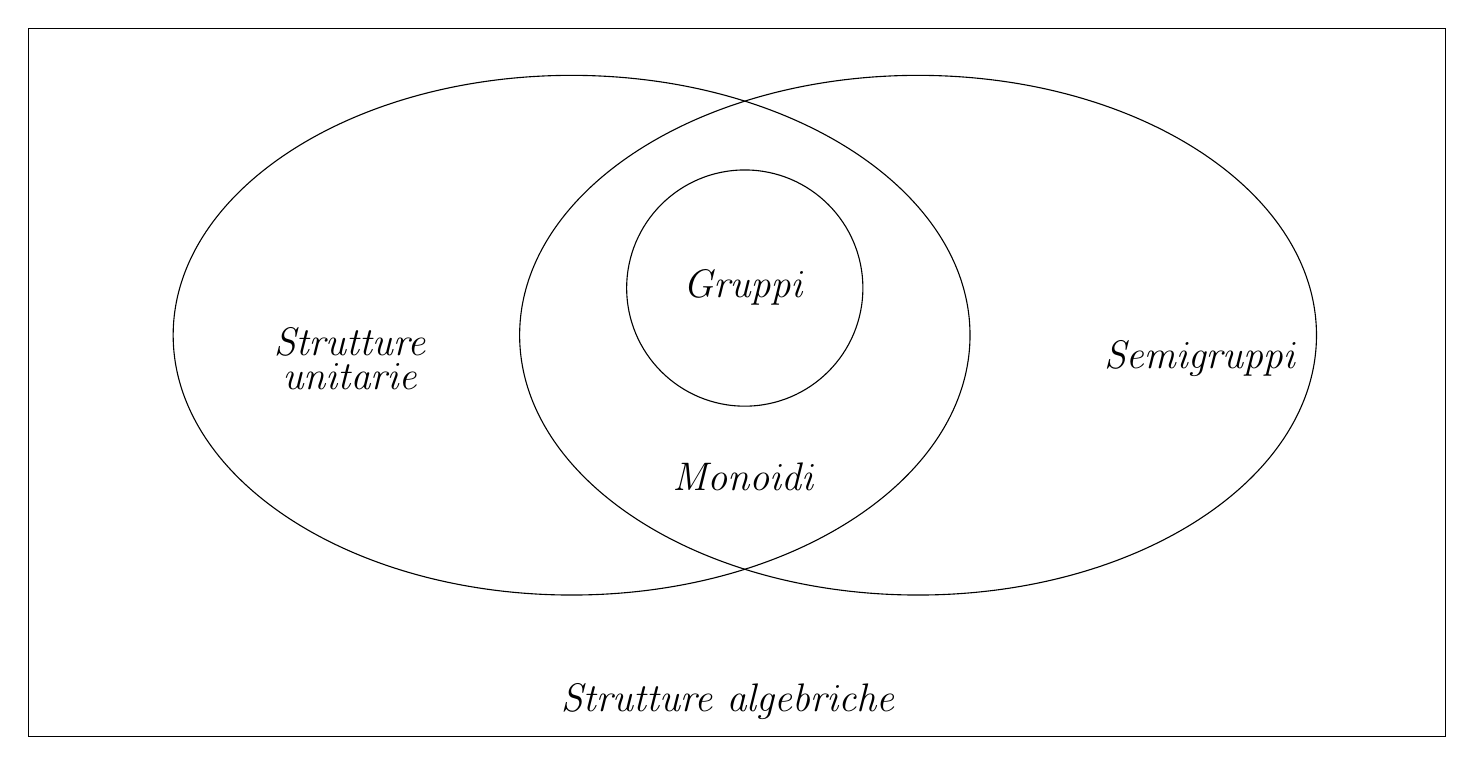
\begin{tikzpicture}
		% Define the size of the rectangle
		\draw[draw=black] (9.1, 6.2) rectangle ++(18, 9);
		
		% Calculate the center of the rectangle and move it on the y-axis
		\coordinate (center) at (16, 11.3);
		
		\begin{scope}
			% Create the first circle
			\draw[xscale=2.3, yscale=1.5] (center) circle (2.2cm);
		\end{scope}
		
		
		
		\begin{scope}
			% Calculate the position for the third circle relative to the center and move it on the y-axis
			\coordinate (thirdCircle) at ([xshift=2.2cm, yshift=0.6cm] center);
			
			% Create the third circle
			\draw (thirdCircle) circle (1.5cm);
			
			% Text inside the third circle
			\node[align=center, text width=5cm,] at (thirdCircle) {\Large{\textit{Gruppi}}};
		\end{scope}
		
		\begin{scope}
			% Calculate the position for the second circle relative to the center
			% Reduce the xshift to make the circles overlap more
			\coordinate (secondCircle) at ([xshift=4.4cm] center);
			
			% Create the second circle
			\draw[xscale=2.3, yscale=1.5] (secondCircle) circle (2.2cm);
		\end{scope}
		% Text
		\begin{scope}
			\node[align=center, xshift=13.2cm, yshift=11cm] {\Large{\textit{Strutture}}\\ \Large{\textit{unitarie}}};
			\node[below] at (18, 7) {\Large{\textit{Strutture algebriche}}};
			\node[align=center, xshift=24cm, yshift=11cm] {\Large{\textit{Semigruppi}}};
			\node[align=center, xshift=18.2cm, yshift=9.5cm] {\Large{\textit{Monoidi}}};
		\end{scope}
	\end{tikzpicture}
	\captionof{figure}{Strutture algebriche ad una singola operazione interna}
\end{center}

\marker{yellow!50}{yellow!20!black}{Per \textbf{gruppoide} si intende una struttura $(A,\bot)$ dotata di una operazione interna.\index{Gruppoide}}

\begin{center}
	\begin{tikzpicture}[every text node part/.style={align=center},rec/.style={fill=blue!20!white,rectangle,minimum height=1.5cm,minimum width=5cm},>=latex]
		\node[rec] (g) {\textbf{Gruppoide} $(A,\bot)$};
		\node[rec, below=1cm of g] (s) {\textbf{Semigruppo} \\ $\bot$ associativa};
		
		\node[rec,right=5cm of s](sa){\textbf{Semigruppo abeliano} \\ $\bot$ associativa \\ $\bot$ commutativa};
		\node[rec,below=1cm of sa] (ma){\textbf{Monoide abeliano} \\ $\bot$ associativa \\ $\exists u \in A (\forall a \in A (a \bot u=u \bot a = a))$ \\ $\bot$ commutativa};
		\node[rec,below=1cm of ma](ga){\textbf{Gruppo abeliano} \\ $\bot$ associativa \\ $\exists u \in A \bigl(\forall a \in A (a \bot u=u \bot a = a)\bigr)$ \\ $\forall x \in A \bigl(\exists x' (x \bot x'=u)\bigr)$ \\ $\bot$ commutativa};
		\node[rec, below=1cm of s](m){\textbf{Monoide} \\ $\bot$ associativa \\ $\exists u \in A (\forall a \in A (a \bot u =u \bot a =  a))$ };
		\node[rec,below=1.5cm of m](gr){\textbf{Gruppo} \\ $\bot$ associativa \\ $\exists u \in A \bigl(\forall a \in A (a \bot u=u \bot a = a)\bigr)$ \\ $\forall x \in A \bigl(\exists x' (x \bot x'=u)\bigr)$};
		\draw[->] (g) to node[midway,right]{$\bot$ associativa}(s);
		\draw[->] (s) to node[midway,right]{Esiste elemento neutro}(m);
		\draw[->] (m) to node[midway,right]{Esistono simmetrici}(gr);
		\draw[->](s) to node[midway,above]{$\bot$ commutativa}(sa);
		\draw[->](m) to node[midway,above]{$\bot$ commutativa}(ma);
		\draw[->](gr) to node[midway,above]{$\bot$ commutativa}(ga);
		\draw[->] (sa) to node[midway,right]{Esiste elemento neutro}(ma);
		\draw[->] (ma) to node[midway,right]{Esistono simmetrici}(ga);
	\end{tikzpicture}
	\captionof{figure}{Caratterizzazione delle strutture ad una singola operazione interna}
\end{center}

\section{Anelli}

\begin{defbox}{Anello}\index{Anello}
	Un \textbf{anello} è un insieme $A$ dotato di due operazioni $+$, $\cdot$ (che saranno sempre chiamate ``somma'' e ``prodotto''), che soddisfano le seguenti proprietà:
	\begin{enumerate}
		\item $(G,+)$ è un gruppo abeliano:
		\begin{enumerate}
			\item $+$ è associativa
			\item $+$ è commutativa
			\item Esiste l'elemento neutro rispetto a $+$ ed è denotato con $0_{G}$
			\item Per ogni $x \in G$ esiste $-x \in G$ tale che $x+(-x)=0_{G}$.
		\end{enumerate}
		\item $(G,\cdot)$ è un semigruppo
		\item L'operazione $\cdot$ è distributiva rispetto a $+$:
		\begin{displaymath}
			\forall a,b,c \in A \begin{cases}
				a \cdot (b+c) = ab + ac \\
				(a+b)c = ac + bc
			\end{cases}
		\end{displaymath}
	\end{enumerate}
	Se anche l'operazione $\cdot$ è commutativa allora l'anello si dice \textbf{abeliano}. Se esiste l'elemento neutro per la moltiplicazione\footnote{Quindi $(A,\cdot)$ è un monoide} indicato con $1_{A}$ allora l'anello si dice \textbf{unitario}.
\end{defbox}
\begin{example}
	Sono anelli, con le usuali operazioni di somma e prodotto, gli insiemi numerici $\mathbb{R}, \mathbb{Z}, \mathbb{Q}, \mathbb{C}$.
\end{example}
\begin{example}
	Dato l'insieme $E=\{a,b,c\}$ consideriamo l'insieme delle parti $\mathcal{P}(E)$: $$\mathcal{P}(E)= \{\emptyset, \{a\}, \{b\}, \{c\}, \{a,b\}.\{b,c\},\{a,c\},E\}$$ Consideriamo in tale insieme le due operazioni di differenza simmetrica $\triangle$ e di intersezione $\cap$. È facile verificare che la struttura $(\mathcal{P}(E),\triangle,\cap)$ è un anello:
	\begin{enumerate}
		\item L'operazione $\triangle$ è associativa e commutativa;
		\item Esiste l'elemento neutro rispetto a $\triangle$, ovvero l'elemento: $\emptyset$: $\forall x \in \mathcal{P}(E) \bigl(a \triangle \emptyset = \emptyset \triangle a = a\bigr)$;
		\item Ogni elemento $ a \in \mathcal{P}(E)$ ha come simmetrico se stesso rispetto a $\triangle$: $a \triangle a = (a \cup a ) \setminus (a \cap a) = \emptyset$. Quindi $(\mathcal{P}(E),\triangle)$ è un gruppo;
		\item L'operazione $\cap$ è associativa e commutativa;
		\item Esiste l'elemento neutro rispetto a $\cap$, ovvero $E$ e vale: $\forall a \in \mathcal{P}(E) \bigl(a \cap e = e \cap a = a \bigr)$;
		\item L'intersezione è distributiva rispetto alla differenza simmetrica: $$\forall a,b,c \in \mathcal{P}(E) \bigl(a \cap (b \triangle c) = (a \cap b) \triangle (a \cap c)\bigr)$$
	\end{enumerate}
	Pertanto la struttura $(\mathcal{P}(E),\triangle,\cap)$ è un anello commutativo unitario. Tale anello prende il nome di \textbf{anello di Boole}.
\end{example}



\subsection{Regole di calcolo in un anello}
Dagli assiomi che definiscono la struttura di anello, seguono di fatto molte di quelle proprietà delle operazioni che utilizziamo familiarmente nel caso di anelli numerici. Le elenchiamo nelle seguenti proposizioni: la prima riguarda la somma, e non è altro che la \textbf{legge di cancellazione}, valida in qualsiasi gruppo; la seconda riguarda il prodotto (si osservi come sia fondamentale la proprietà distributiva).

\begin{propbox}	
	Sia $A$ un anello. Allora, per ogni $a,b,c \in A$:
	\begin{equation}
		a+b = a+c  \implies b=c
	\end{equation}
\end{propbox}
\begin{proof}
	Siano per ogni $a,b,c \in A$, tali che $a+b=a+c$ e sia $a'\in A$ tale che $a'+a=0_{A}$. Allora:
	\begin{align*}
		b &= 0_{A}+b  & \text{\textcolor{gray}{(elemento neutro della somma)}}\\
		&= (a+a')+b & \text{\textcolor{gray}{(elemento opposto)}}\\
		&= a' + (a+b) & \text{\textcolor{gray}{(proprietà associativa)}}\\
		&=a' + (a+c) & \text{\textcolor{gray}{(per ipotesi)}} \\
		&=(a'+a)+c  =0_{A}+c =c \\
	\end{align*}
\end{proof}

Supponiamo ora che $0'_{A}$ sia un elemento neutro per la somma. Allora:
$	0'_{A} = 0'_{A}+0_{A}=0_{A}$. Infine, se $a'$ e $a''$ sono opposti dell'elemento $a$, allora $a+a'=0_{A}=a+a''$ e quindi, per quanto provato sopra, $a'=a''$. Se $a$ e $b$ sono elementi dell'anello $A$, si adotta la seguente notazione: $a-b=a+(-b)$. Nel caso del prodotto invece si è soliti scrivere direttamente: $a \cdot b = ab$.


\begin{propbox}
	Sia $A$ un anello unitario, e siano $a,b \in A$ allora:
	\begin{enumerate}
		\item Esiste un unico elemento neutro per il prodotto
		\item $a \cdot 0_{A}=0_{A} \cdot a=0_{A}$
		\item $a(-b)=-(ab)=(-a)b$
		\item $(-a)(-b)=ab$
	\end{enumerate}
\end{propbox}

\begin{proof}
	$(1)$ Siano $1_{A}$ e $1'_{A}$ elementi neutri per il prodotto. Allora, analogamente a quanto visto per l'addizione:
	\begin{displaymath}
		1'_{A} = 1'_{A} \cdot 1_{A} = 1_{A}
	\end{displaymath}
	
	$(2)$ Sia $c = a 0_{A}$. Allora, applicando la proprietà distributiva:
	\begin{align*}
		c &= a 0_{A} & \text{\textcolor{gray}{(per ipotesi)}}\\
		&= a(0_{A}+0_{A}) & \text{\textcolor{gray}{(idempotenza)}}\\
		&= a0_{A} +a0_{A} & \text{\textcolor{gray}{(proprietà distributiva)}}\\
		&= c+c\\
	\end{align*}
	e quindi $c=c+c-c=c-c = 0_{A}$. Analogamente si dimostra che $0_{a} a = 0_{A}$.
	
	$(3)$ Proviamo che $a(-b)=-(ab)$. Applicando la proprietà distributiva ed il punto 2:
	\begin{align*}
		a(-b)+ab&=a(-b+b)=a0_{A}=0_{A}
	\end{align*}
	e quindi $a(-b) =-(ab)$. Analogamente si dimostra che $(-a)b=-(ab)$.
	
	$(4)$ Per il punto 3 si ha:
	\begin{align*}
		(-a)(-b)&=-(a(-b))\\
		&=-(-(ab))\\
		&=ab
	\end{align*}
\end{proof}

Anche per un generico anello è possibile definire l'elevazione a potenza per un numero intero.  In generale, in un anello non commutativo, $A$ non è detto che, dati $a,b \in A$ e $n \in \mathbb{N}$ valga $(ab)^{n}=a^{n}b^{n}$. Tuttavia, non è difficile provare che se $ab=ba$ allora si ha, per ogni $n \in \mathbb{N}$, $(ab)^{n}=a^{n}b^{n}$. In particolare, questa ulteriore proprietà delle potenze sussiste negli anelli abeliani, nei quali vale il seguente teorema:

\begin{teorbox}
	[del binomio di Newton]\index{Binomio di Newton}
	Sia $A$ un anello commutativo, e siano $a,b \in A$. Per ogni $n \in \mathbb{N}$:
	\begin{equation}
		(a+b)^{n}= \sum_{i=0}^{n}\binom{n}{i}a^{n-i}b^{i}
	\end{equation}
\end{teorbox}

Questa formula non vale se l'anello non è commutativo. Per verificarlo basta osservare ciò che accade se si prova a calcolare $(a+b)^{3}$:
\begin{align*}
	(a+b)^{3} &= (a+b)(a+b)(a+b) \\
	&= a(a+b)(a+b) + b(a+b)(a+b) 	\\
	&= a(a(a+b) +b(a+b)) + b(a(a+b)+b(a+b))\\
	&= a(aa+ab +ba+bb) + b(aa+ab+ba+bb) \\
	&= aaa+aab+aba+abb + baa +bab + bba + bbb \\
\end{align*}

Se l'anello fosse commutativo si potrebbero unire i fattori $(aab+aba+baa)$ come $3a^{2}b$ e ottenere la formula indicata dal binomio di Newton ma essendo $ab \neq ba$ questo non è possibile e tutti i fattori sono uno diverso dall'altro.

\begin{defbox}{Sottoanello}\index{Sottoanello}
	Un sottoinsieme non vuoto $S$ di un anello $A$ che sia chiuso rispetto alle due operazioni di $A$ si dice \textbf{sottoanello} di $A$.
\end{defbox}

\subsection{Tipologie di anello}
La nozione di cancellabilità, come quella di invertibilità, riveste una grande importanza in teoria degli anelli. In questo contesto una prima precisazione, per quanto ovvia, è necessaria: \textit{ogni elemento di un anello è simmetrizzabile, quindi anche cancellabile, rispetto all'operazione additiva}, dunque quando si parla di elementi cancellabili o simmetrizzabili in un anello è all’operazione moltiplicativa che si fa riferimento. 

Nei paragrafi precedenti abbiamo provato alcune proprietà degli anelli, che per $\mathbb{Z}$ siamo abituati a considerare ``naturali''. Ora, $\mathbb{Z}$ soddisfa anche altre proprietà, quali il fatto che il prodotto di due elementi diversi da zero è diverso da zero. Questa legge non discende dagli assiomi di anello, esistono infatti anelli in cui questa legge non vale.

\begin{defbox}{Divisore dello zero}\index{Divisore!dello zero}
	Sia $(A,+,\cdot)$ un anello e sia $a \in A$. Allora:
	\begin{itemize}
		\item $a$ è un \textbf{divisore sinistro dello zero} in $A$ se e soltanto se esiste un elemento $b \in A$ tale che $b \neq 0_{A}$ e $ab=0_{A}$.
		\item $a$ è un \textbf{divisore destro dello zero} in $A$ se e soltanto se esiste un elemento $b \in A$ tale che $b \neq 0_{A}$ e $ba=0_{A}$.
		\item $a$ è un \textbf{divisore dello zero} in $A$ se e soltanto se esiste un elemento $b \in A$ tale che $b \neq 0_{A}$ e $ab=ba=0_{A}$.
	\end{itemize}
\end{defbox}

\begin{example}
	Un esempio di divisori dello zero si può trovare negli anelli di matrici; ad esempio, in $(M_{2}(\mathbb{R}),+,\cdot)$ ovvero l'anello delle matrici\index{Matrice} quadrate di dimensione $2$ con le operazioni di somma e prodotto righe per colonne si ha:
	\begin{displaymath}
		\begin{bmatrix}
			0 & 1 \\
			0 & 1
		\end{bmatrix}
		\begin{bmatrix}
			1 & 1 \\
			0 & 0
		\end{bmatrix}
		=
		\begin{bmatrix}
			0 & 0 \\
			0 & 0 \\
		\end{bmatrix}
	\end{displaymath}
\end{example}

\begin{teorbox}\label{thm:car_divisori_zero}
	Per ogni elemento $a \in A$ si ha che:
	\begin{itemize}
		\item $a$ è un divisore sinistro dello zero in $A$ se e soltanto se $a$ non è cancellabile a sinistra in $(A, \cdot)$;
		\item $a$ è un divisore destro dello zero in $A$ se e soltanto se $a$ non è cancellabile a destra in $(A, \cdot)$;
		\item $a$ è un divisore dello zero in $A$ se e soltanto se non è cancellabile in $(A,\cdot)$.
	\end{itemize}
	
\end{teorbox}

\begin{proof}
	Dimostriamo la prima delle equivalenze logiche, la seconda equivalenza si dimostra in maniera analoga mentre la terza discende dalla veridicità delle prime due equivalenze.
	
	$\implies)$ Sia $a$ un divisore sinistro dello zero in $A$. Allora, per definizione, esiste un elemento $b \in A$ tale che $ab=0_{A} \neq b$.  Chiaramente vale: $0_{A}= a \cdot 0_{A}$ eppure l'equivalenza $ab=a0_{A}$ non implica che $b = 0_{A}$. Quindi $a$ non è cancellabile a sinistra.
	
	$\impliedby)$ Se $a$ non è cancellabile a sinistra in $(A,\cdot)$ allora esistono $u$ e $v$ in $A$ tale che $au=av$ e $u \neq v$. Per tali $u$ e $v$:
	\begin{align*}
		au &= av\\
		au - av &= 0_{A}\\
		a(u-v) &= 0_{A}\\
	\end{align*}
	e quindi $a$ è un divisore sinistro dello zero.
\end{proof}


\begin{teorbox}
	In un anello con più di un elemento, lo zero ($0_{A}$) è un divisore dello zero.
\end{teorbox}

\begin{proof}
	Sia $|A|>1$ allora esiste un elemento $b \in A \setminus \{0_{A}\}$ per il quale $0_{A}= 0_{A}= b 0_{A}$ e quindi $0_{A}$ risulta un divisore dello zero. Ovviamente se $|A|=1$ le operazioni di somma e prodotto coincidono in quanto si ha $0_{A}=1_{A}$.
\end{proof}

\begin{defbox}{Anello integro}\index{Anello!integro}
	Un anello si dice \textbf{integro} se in esso vale la legge di annullamento del prodotto.
	
\end{defbox}

Con la terminologia appena introdotta, possiamo riformulare questa condizione in questo modo: un anello è integro se e solo se non ha divisori propri dello zero. Per quanto appena dimostrato, ciò equivale anche a dire che nell'anello in questione ogni elemento diverso da zero è cancellabile.

\begin{propbox}[Legge di annullamento del prodotto]\label{annullamento_prodotto}
	Sia $A$ un anello integro e siano $a,b \in A$ due elementi qualsiasi. Si ha allora:
	\begin{equation}
		ab = 0 \implies (a=0 \lor b=0)
	\end{equation}
\end{propbox}

\begin{defbox}{Dominio di integrità}\index{Dominio!di integrità}
	Un anello si dice un \textbf{dominio di integrità} se è un anello integro commutativo unitario.
\end{defbox}

\begin{propbox}[Legge di cancellazione]\index{Legge!di cancellazione}
	Sia $A$ un dominio di integrità, allora per ogni $a,b \in A$ e per ogni $c \neq 0_{A}$ si ha:
	\begin{equation}
		ac=bc  \implies a=b
	\end{equation}
	Possiamo formularne la definizione in uno qualsiasi dei seguenti modi, tra loro equivalenti: un dominio
	di integrità è:
	\begin{itemize}
		\item un anello commutativo integro;
		\item un anello commutativo in cui vale la legge di annullamento del prodotto;
		\item un anello commutativo in cui ogni elemento diverso da zero è cancellabile.
	\end{itemize}
\end{propbox}
\begin{teorbox}
	Un anello $(A,+,\cdot)$ è un dominio di integrità se è privo di divisori dello zero.
\end{teorbox}
\begin{proof}
	\begin{itemize}
		\item[$\implies$] Se l'anello è un dominio di integrità, per la Proposizione \ref{annullamento_prodotto}  vale la legge di annullamento del prodotto. Per assurdo, sia $x \in A$ un divisore dello zero, allora:
		\begin{align*}
			\exists y \in A \setminus \{0_{A}\}\bigl(xy=0\bigr)
		\end{align*}
	e dunque, per la legge di annullamento del prodotto, deve essere $x=0_{A} \lor y=0_{A}$ che va contro le ipotesi che siano entrambi non nulli. Quindi $A$ è privo di divisori dello zero.
	\item[$\impliedby$] Se nessun elemento è divisore dello zero, allora tutti gli elementi sono cancellabili per il Teorema \ref{thm:car_divisori_zero}. Dunque, se consideriamo:
	\begin{align*}
		\forall x,y \in A \bigl( x \neq 0_{A} \land xy = 0_{A} \implies y = 0_{A} \bigr)
	\end{align*}
Quindi $A$ è un dominio di integrità, come volevasi dimostrare.
	\end{itemize}
\end{proof}
\begin{defbox}{Corpo}\index{Corpo}
	Un anello unitario $A$ si dice \textbf{corpo} se ogni elemento non nullo di $A$ è invertibile.
\end{defbox}

\begin{defbox}{Campo}\index{Campo}
	Un \textbf{campo} è un corpo commutativo, ovvero un anello abeliano in cui ogni suo elemento non nullo è invertibile.
\end{defbox}


\begin{propbox}
	Ogni campo è un dominio di integrità.
\end{propbox}

\begin{proof}
	Un campo è un corpo commutativo, ed un corpo è un anello unitario. Un anello commutativo unitario è dominio di integrità se e soltanto
	se è privo di divisori dello zero. Ogni elemento di un campo, eccetto lo	zero, è invertibile, e dunque cancellabile. Un elemento cancellabile non può essere divisore dello zero, e quindi non esistono divisori dello zero. Dunque il campo è dominio di integrità.
\end{proof}

Non vale il viceversa, non tutti i domini di integrità sono dei campi. Ad esempio $(\mathbb{Z},+,\cdot)$ è un dominio di integrità ma non è un campo in quanto, ad esempio, il numero 2 non ha un inverso moltiplicativo in $\mathbb{Z}$. \textit{Ogni dominio di integrità finito}, però, \textit{risulta essere un campo}. La ragione sta nel fatto che in un dominio di integrità finito, ogni elemento non nullo deve necessariamente avere inverso moltiplicativo. Questo può essere dimostrato con un argomento di tipo combinatorio. Sia $D$ un dominio di integrità con $n$ elementi. Consideriamo l'elemento $a \in D$ con $a \neq 0_{D}$. La funzione $f: D \rightarrow D$ definita da $f(x) = ax$ è iniettiva. Infatti:
	\begin{align*}
		\forall x,y \in D (f(x) = f(x) \iff ax = ay)
	\end{align*}
e poiché $D$ è un dominio di integrità, vale la legge di cancellazione, cioè: $x=y$. Essendo $f$ una funzione iniettiva tra due insiemi equipotenti questa risulta essere anche suriettiva. Dunque deve esistere un elemento $b \in D$ tale che $ab= 1_{D}$ e $b$ risulta essere $a^{-1}$. Questo dimostra che ogni elemento non nullo ha un inverso moltiplicativo e $D$ è un campo.

\begin{center}
	\begin{tikzpicture}
		[every text node part/.style={align=center},rec/.style={fill=blue!20!white,rectangle,minimum height=1.5cm,minimum width=3cm},>=latex]
		\node[rec,name=a]{\textbf{Anello} \\ $(A,+,\cdot)$};
		\node[rec,name=a1, below of=a, yshift=-1cm]{$S \neq \emptyset$};
		\node[rec,name=a2,right of=a1,xshift=3cm]{$(S,+)$ è un gruppo};
		\node[rec,name=a3,right of=a2,xshift=6cm]{$\cdot$ è associativa \\ $\cdot$ è distributiva rispetto a $+$};
		\node[rec,name=ac,below of=a3, yshift=-2cm]{\textbf{Anello commutativo}};
		\node[rec,name=au,below of=a2, yshift=-2cm]{\textbf{Anello unitario}};
		\node[rec,name=c,below of=au,yshift=-2cm]{\textbf{Corpo}};
		\node[rec,name=d,below of=ac,yshift=-2cm]{\textbf{Dominio di integrità}};
		\node[rec,name=k,below of=c,yshift=-2cm]{\textbf{Campo}};
		\draw[->,>=stealth](a)--(a1);
		\draw[->,>=stealth](a) -| (a2);
		\draw[->,>=stealth](a) -| (a3);
		\draw[->,>=stealth](a3) to node[right,midway]{$\cdot$ è commutativa} (ac);
		\path [draw, >=latex] (a3) |- ($(a3)+(0,-1.5)$) -| node[above,midway]{Se esiste $1_{A}$}(au);
		\draw[->,>=stealth](ac) to node[right,midway]{Se non ci sono \\ divisori dello zero}(d);
		\path [draw, >=latex] (au) -- ($(au)+(2,0)$) |-  node[midway,right]{Se non ci sono \\ divisori dello zero}(d);
		\draw[->](au) to node[left,midway]{Se ogni elemento\\ non nullo è invertibile rispetto a $\cdot$}(c);
		\draw[->](c) to node[left,midway]{Se $\cdot$ è commutativa}(k);
		\draw[->,>=stealth](d) |- node[right,midway]{Se ogni elemento \\ non nullo è invertibile \\ rispetto a $\cdot$}(k);
	\end{tikzpicture}
	\captionof{figure}{Caratterizzazione dei corpi}
\end{center}
\newpage
\section{Esercizi svolti}
\begin{exsbox}
	Sia $A=\{1,2\}$ e consideriamo l'operazione di intersezione nell'insieme delle parti di A:
	\begin{displaymath}
		\cap : \mathcal{P}(A) \times \mathcal{P}(A) \longrightarrow \mathcal{P}(A)
	\end{displaymath}
	Si rappresenti la relativa tavola di Cayley.
\end{exsbox}
\paragraph*{Svolgimento.} Si ha:
\begin{center}
	\begin{tblr}{
			hlines,
			vlines,
			row{1}={primary!80!white},
			column{1}={primary!80!white},
			cells={mode=math}
		}
		\cap & \varnothing & \{1\} & \{2\} & A \\
		\varnothing & \varnothing & \varnothing & \varnothing & \varnothing \\
		\{1\} & \varnothing & \{1\} & \varnothing & \{1\} \\
		\{2\} & \varnothing & \varnothing & \{ 2\} & \{2\} \\
		A & \varnothing & \{1\} & \{2\} & A \\
	\end{tblr}
\end{center}
\begin{flushright}
	\blacksquare
\end{flushright}
\begin{exsbox}
	Vero o falso? Per ogni insieme non vuoto $S$ ed ogni operazione binaria $\ast$ in S,...
	\begin{enumerate}
		\item In $S$ esiste sempre un elemento neutro a destra o un elemento neutro a sinistra;
		\item Se $\ast$ è commutativa, tutti gli elementi neutri a destra in $(S,\ast)$ sono anche neutri a sinistra;
		\item Se $\ast$ è commutativa, in $S$ esiste al massimo un elemento neutro a sinistra;
		\item Se $a$ e $b$ sono due elementi neutri a sinistra distinti in $(S, \ast)$, in $(S,\ast)$ non esistono elementi neutri a destra.
	\end{enumerate}
\end{exsbox}
\paragraph*{Svolgimento.} Sia $(S,\ast)$ un'arbitraria struttura algebrica.
\begin{enumerate}
	\item Falso. Ad esempio nell'insieme degli interi maggiori di 1 con l'operazione della moltiplicazione non esiste elemento neutro.
	\item Vero. Infatti se esiste un elemento $t \in S$ neutro a destra allora $\forall x \in S (x \ast t = t \ast x = x )$ e quindi $t$ è neutro a sinistra.
	\item Vero. Infatti, posto $u$ l'elemento neutro a sinistra, se esistesse un secondo elemento neutro a sinistra $u'$ si avrebbe:
	\begin{displaymath}
		u' = u \ast u' = u' \ast u = u
	\end{displaymath}
	\item Vero. Infatti se per assurdo esistesse un elemento neutro a destra, detto $u'''$, si avrebbe:
	\begin{displaymath}
		u'  \ast u''' = u'
	\end{displaymath}
	ma anche:
	\begin{displaymath}
		u'' \ast u''' = u''
	\end{displaymath}
	Tuttavia, poiché $u'$ e $u''$ sono elementi distinti si deve avere:
	\begin{displaymath}
		u' \ast u''' = u''' = u'' \ast u'''
	\end{displaymath}
	ma $u'' \neq u'$. \hfill \blacksquare
\end{enumerate}
\begin{exsbox}
	Dato l'insieme $A=\{0,1\}$ scrivere le tavole di Cayley di $(\mathcal{P}(A), \cup)$ e di $(\mathcal{P}(A), \triangle)$.
\end{exsbox}
\paragraph*{Svolgimento.} Si ha:
\begin{center}
	\begin{minipage}{.45\textwidth}
		\centering
		\begin{tblr}{
				hlines,
				vlines,
				row{1}={primary!80!white},
				column{1}={primary!80!white},
				cells={mode=math}
			}
			\cup & \varnothing & \{0\} & \{1\} & A \\
			\varnothing & \varnothing & \{0\} & \{1\} & A \\
			\{0\} & \{0\} & \{0\} & A & A \\
			\{1\} & \{1\} & A & \{1\} & A \\
			A & A & A & A & A
		\end{tblr}
	\end{minipage}
	\hfil
	\begin{minipage}{.45\textwidth}
		\centering
		\begin{tblr}
			{
				hlines,
				vlines,
				row{1}={primary!80!white},
				column{1}={primary!80!white},
				cells={mode=math}
			}
			\triangle & \varnothing & \{0\} & \{1\} & A \\
			\varnothing & \varnothing & \{0\}& \{1\} & A \\
			\{0\} & \{0\} & \varnothing & A & \{1\} \\
			\{1\} & \{1\} & A & \varnothing & \{0\} \\
			A & A & \{1\} & \{0\} & \varnothing
		\end{tblr}
	\end{minipage}
\end{center}
\begin{flushright}
	\blacksquare
\end{flushright}
\begin{exsbox}
	Studiare le operazioni binarie qui elencate, stabilendo per ciascuna di essere se è commutativa e se è associativa, e determinando gli elementi neutri a sinistra, a destra, neutri delle strutture da esse definite:
	\begin{enumerate}
		\item $\alpha: (a,b) \in \mathbb{N} \times \mathbb{N} \mapsto a 10^{b} \in \mathbb{N}$
		\item $\beta:(a,b) \in \mathbb{Z} \times \mathbb{Z} \mapsto -ab \in \mathbb{Z}$
		\item $\gamma:(a,b) \in \mathbb{Q} \times \mathbb{Q} \mapsto \frac{(a+b)}{2} \in \mathbb{Q}$
		\item $\delta: (a,b) \in \mathbb{Z} \times \mathbb{Z} \mapsto 2ab \in \mathbb{Z}$
		\item $\epsilon:(a,b) \in \mathbb{Q} \times \mathbb{Q} \mapsto 2ab \in \mathbb{Q}$
		\item $ \zeta : (a,b) \in \mathbb{Z} \times \mathbb{Z} \mapsto a+b+2 \in \mathbb{Z}$
		\item $\eta : (a,b) \in \mathbb{N} \times \mathbb{N} \mapsto a(b^{a+b}+3ab^{2})+1 \in \mathbb{N}$
		\item $\theta: (a,b) \in \mathcal{P}(\mathbb{Z})\times \mathcal{P}(\mathbb{Z}) \mapsto (a \cap \mathbb{N})\cup b \in \mathbb{Z}$
		\item $\iota : (a,b) \in \mathcal{P}(\mathbb{Z})\times \mathcal{P}(\mathbb{Z}) \mapsto a \cup b \cup \{1\} \in \mathbb{Z}$
	\end{enumerate}
\end{exsbox}
\paragraph*{Svolgimento.}
Si ha:
\begin{enumerate}
	\item L'operazione non è commutativa. Infatti:
	\begin{displaymath}
		\exists a,b \in \mathbb{N} (a 10^{b} \neq b 10^{a})
	\end{displaymath}
	ad esempio $(0,1)$.
	L'operazione non è associativa. Per essere associativa deve valere:
	\begin{displaymath}
		\forall a,b,c \in \mathbb{N}\quad  \bigl(	a \ \alpha \ (b \ \alpha \ c) = (a \ \alpha \  b) \ \alpha \ c  \bigr)
	\end{displaymath}
	ovvero:
	\begin{displaymath}
		a \cdot 10 ^{b \cdot 10 ^{c}} = a \cdot 10 ^{b+c}
	\end{displaymath}
	Scritto così è facile trovare una terna controesempio. Infatti sia $(1,1,2)$ si ha:
	\begin{displaymath}
		\begin{array}{l}
			a \cdot 10 ^{b \cdot 10 ^{c}} = 1 \cdot 10^{1 \cdot 10^{2}} = 10 ^{100}\\
			a \cdot 10 ^{b+c} = 1 \cdot 10^{1+2}= 1000
		\end{array}
	\end{displaymath}
	Si ha inoltre che $0 \in \mathbb{N}$ è neutro a destra rispetto ad $\alpha$, infatti:
	\begin{displaymath}
		\forall a \in \mathbb{N} (a \ \alpha \ 0 = a 10^{0} = a)
	\end{displaymath}
	A questo punto, per il \hyperlink{thm:neutro}{Teorema di unicità dell'elemento neutro}, se esiste un elemento neutro a sinistra deve essere proprio $0$ ma è evidente che $0$ non è neutro a sinistra.
	\item L'operazione è commutativa e associativa. Infatti:
	\begin{displaymath}
		\forall a,b \in \mathbb{Z} \bigl( a \ \beta \ b = -ab = -ba = b \ \beta \ a  \bigr)
	\end{displaymath}
	e
	\begin{displaymath}
		\forall a,b,c \in \mathbb{Z} \bigl(a \ \beta \ (b \ \beta \ c) = a \ \beta \ (-bc) = -(a(-bc))= abc\bigr)
	\end{displaymath}
	ma anche:
	\begin{displaymath}
		\forall a,b,c \in \mathbb{Z} \bigl((a \ \beta \ b) \beta \ c = (-ab) \ \beta \ c = -(-ab)c=abc\bigr)
	\end{displaymath}
	L'elemento $-1$ risulta neutro rispetto a $\beta$, infatti:
	\begin{displaymath}
		\forall b \in \mathbb{Z} \bigl(-1 \ \beta \ b = -(-1b)=b = -(b(-1))=b \ \beta \ -1 \bigr)
	\end{displaymath}
	\item L'operazione risulta commutativa:
	\begin{displaymath}
		\forall a,b \in \mathbb{Q} \bigl( a \ \gamma \ b = \frac{a+b}{2} = \frac{b+a}{2} = b \ \gamma \ a \bigr)
	\end{displaymath}
	ma non associativa. Infatti:
	\begin{displaymath}
		\forall a,b,c \in \mathbb{Q} \bigl(a \ \gamma \ (b \ \gamma \ c ) = a \ \gamma (\frac{b+c}{2}) = \frac{a+ \frac{b+c}{2}}{2} = \frac{2a+b+c}{4}  \bigr)
	\end{displaymath}
	e \begin{displaymath}
		\forall a,b,c \in \mathbb{Q} \bigl((a \ \gamma \ b) \ \gamma \ c = \frac{\frac{a+c}{2}+c}{2}= \frac{a+b+2c}{4}\bigr)
	\end{displaymath}
	presa la terna $(1,1,0)$ si ha:
	\begin{align*}
		\frac{2a+b+c}{4}&=\frac{2+1+0}{4}\\
		&=\frac{3}{4}
	\end{align*}
	e
	\begin{align*}
		\frac{a+b+2c}{4}&=\frac{1+1+0}{4}\\
		&=\frac{2}{4}=\frac{1}{2}
	\end{align*}
	Per esistere elemento neutro a destra deve esistere un elemento $t \in \mathbb{Q}$ tale che:
	\begin{displaymath}
		\forall a \in \mathbb{Q} (t \ \gamma \ a = a)
	\end{displaymath}
	ovvero:
	\begin{align*}
		\frac{a+t}{2}&=a \\
		a+t &= 2a \\
		t &= 2a-a \\
		t&=a
	\end{align*}
	ma non esiste $t \in \mathbb{Q}$ uguale ad ogni numero razionale. Quindi non esiste elemento neutro a destra. Analogamente a sinistra.
	\item L'operazione $\delta$ è commutativa e associativa. Infatti:
	$$ \forall a,b \in \mathbb{Z} \bigl( a \ \gamma \ b = 2ab = 2ba = b \ \delta \ a\bigr) $$
	e:
	\begin{displaymath}
		\begin{array}{l}
			\forall a,b,c \in \mathbb{Z} \bigl( a \ \delta \ (b \ \delta \ c) = a \ \delta \ (2bc) = 4abc \bigr)\\
			\forall a,b,c \in \mathbb{Z} \bigl((a \ \delta \ b) \delta c = (2ab) \ \delta \ c = 4abc \bigr)
		\end{array}
	\end{displaymath}
	Non esiste elemento neutro rispetto a $\delta$, infatti se esistesse un elemento neutro a destra $t \in \mathbb{Z}$ si deve avere:
	\begin{eqnarray*}
		a \ \delta \ t &=& a \\
		2at &=& a \\
		t &=& \frac{a}{2a}=\frac{1}{2} \notin \mathbb{Z}
	\end{eqnarray*}
	\item A differenza di $\delta$, l'operazione $\epsilon$ è commutativa, associativa e gode di elemento neutro.
	\item L'operazione è commutativa. Infatti, per ogni $a,b \in \mathbb{Z}$ si ha:
	\begin{displaymath}
		a \ \zeta \ b = a+b+2 = b+a+2 = b  \ \zeta  \ a
	\end{displaymath}
	Per verificare l'associatività deve essere, qualsiasi siano gli elementi $a,b,c \in \mathbb{Z}$:
	\begin{displaymath}
		\begin{cases}
			a \zeta (b \ \zeta \ c) = a \ \zeta \ (b+c+2) = a+(b+c+2)+2=a+b+c+4 \\
			(a \ \zeta \ b) \ \zeta \ c = c \ \zeta \ (a \ \zeta \ b) =c + a + b +4
		\end{cases}
	\end{displaymath}
	quindi $\zeta$ è associativa.
	Per trovare l'elemento neutro partiamo dalla definizione :
	\begin{displaymath}
		\forall a \in \mathbb{Z} \bigl( a \ \zeta \ u = a  \iff a+u+2=a \bigr)
	\end{displaymath}
	L'elemento $-2 \in \mathbb{Z}$ è neutro quindi rispetto a $\zeta$.
	\item L'operazione non è associativa, non è commutativa e non ha elemento neutro. Davanti a formule poco maneggevoli è utile provare cercando terne che negano le proprietà cercate. Infatti data la coppia $(2,3)$ si ha:
	\begin{displaymath}
		2\ \eta \  3 = 2(3^{2+3}+3\cdot2\cdot3^{2})+1=595 \neq 205 = 3(2^{3+2}+3 \cdot 3 \cdot2^{2})+1 = 3 \  \eta \  2
	\end{displaymath}
	e data la terna $(0,0,1)$ si ha:
	\begin{displaymath}
		(0 \ \eta \ 0) \ \eta \ 1 = 5 \neq 1 = 0 \ \eta \ (0 \ \eta \ 1)
	\end{displaymath}
	Per quanto riguarda la verifica dell'esistenza dell'elemento neutro, dalla definizione di elemento neutro a sinistra si ha che $t \in \mathbb{N}$ è neutro a sinistra rispetto a $\eta$ se e solo se:
	\begin{displaymath}
		\forall b \in \mathbb{N} (t \ \eta \ b = b)
	\end{displaymath}
	Osservando la formula dell'operazione si nota che:
	\begin{displaymath}
		\forall a \in \mathbb{N} \bigl( a \ \eta \ 0 = 1 \bigr)
	\end{displaymath}
	da cui si deduce la non esistenza di un elemento neutro. Infatti non esiste un elemento $t \in \mathbb{N}$ tale che $t \ \eta \ 0 = 0$ in quanto abbiamo visto che questo darà sempre 1 come risultato.
	\item L'operazione non è commutativa, seguendo il metodo visto nell'esercizio precedente si può andare per tentativi. Preso $a=\{-1\}\subseteq \mathbb{Z}$ e $b=\{-2,3\}\subseteq \mathbb{Z}$ si ha:
	\begin{displaymath}
		a \ \theta \ b = (a \cap \mathbb{N}) \cup b = (\{-1\}\cap \mathbb{N})\cup b = \varnothing \cup \{-2,3\} = \{-2,3\}
	\end{displaymath}
	\begin{displaymath}
		b \ \theta \ a = (\{-2,3\} \cap \mathbb{N}) \cup \{-1\} = \{3\} \cup \{-1\} = \{-1,3\}
	\end{displaymath}
	mentre per l'associatività, deve valere:
	\begin{displaymath}
		\forall a,b,c \in \mathcal{P}(\mathbb{Z})\bigl( a \ \theta \ (b \ \theta \ c) = (a \ \theta \ b) \ \theta \ c \bigr)
	\end{displaymath}
	Dove:
	\begin{align*}
		a \ \theta \ (b \ \theta \ c) &= a \ \theta \bigl( (b \cap \mathbb{N}) \cup c \bigr) \\
		&= (a \cap \mathbb{N}) \cup \bigl( (b \cap \mathbb{N}) \cup c \bigr)
	\end{align*}
	e:
	\begin{align*}
		(a \ \theta \ b) \ \theta \ c &= \bigl((a \cap \mathbb{N}) \cup b\bigr) \ \theta \ c \\
		&= \Bigl( \bigl((a \cap \mathbb{N}) \cup b\bigr) \cap \mathbb{N} \Bigr) \ \cup \ c \\
		&= \Bigl((a \cap \mathbb{N} \cap \mathbb{N}) \cup (b \cap \mathbb{N} )\Bigr) \ \cup \ c & \text{\textcolor{gray}{Applicando la distributività}} \\
		&= \Bigl( a \cap \mathbb{N} \cup (b \cap \mathbb{N})  \Bigr) \cup c
	\end{align*}
	Quindi vale la proprietà associativa. Se un elemento $a \in \mathcal{P}(\mathbb{Z})$ è neutro a sinistra vale, per ogni $b \in \mathcal{P}(\mathbb{Z})$:
	\begin{displaymath}
		a \ \theta \ b = b
	\end{displaymath}
	ovvero:
	\begin{displaymath}
		(a \cap \mathbb{N}) \cup b = b
	\end{displaymath}
	Data questa condizione si ha sicuramente che:
	\begin{displaymath}
		(a \cap \mathbb{N} = \emptyset) \implies  (a \cap \mathbb{N}) \cup b = b
	\end{displaymath}
	Preso $a \subseteq \mathbb{Z} \wedge a \cap \mathbb{N} \neq \emptyset$ allora $$a \ \theta \ \emptyset = (t \cap \mathbb{N}) \cup \emptyset = t \cap \emptyset \neq \emptyset $$
	Quindi $a$ non è neutro a sinistra in quanto esiste una scelta di $b \in \mathcal{P}(\mathbb{Z})$ che non verifica la condizione: $\emptyset$. Un metodo alternativo per arrivare alla stessa conclusione è quello di osservare che per valere la condizione deve essere:
	\begin{displaymath}
		\forall b \in \mathcal{P}(\mathbb{Z})	\bigl( (a \cap \mathbb{N}) \subseteq b \bigr)
	\end{displaymath}
	quindi deve essere $a \cap \mathbb{N} = \emptyset$. In conclusione $\theta$ ha elementi neutri a sinistra e sono tutte le parti $a \in \mathbb{Z} \setminus \mathbb{N}$. Dati infiniti elementi neutri a sinistra, per il \hyperlink{thm:neutro}{Teorema di unicità dell'elemento neutro} possiamo dire che $(\mathcal{P}(\mathbb{Z}), \theta)$ non ha elementi neutri a destra.
	\item L'operazione è commutativa e associativa per la commutatività e l'associatività dell'unione. Un elemento $t$ è neutro se e solo se, per ogni $b \in \mathcal{P}(\mathbb{Z})$ si ha:
	\begin{displaymath}
		t \ \iota \ b = b \ \iota \ t  = b
	\end{displaymath}
	ovvero:
	\begin{displaymath}
		t \ \iota \ b = t \cup b \cup \{1\} = b
	\end{displaymath}
	ma per ogni scelta di $b$ non esiste un siffatto elemento neutro in quanto il loro composto tramite $\iota$ sarà sempre diverso da $b$. Per convincerci di questa affermazione consideriamo $b= \emptyset$:
	\begin{displaymath}
		t \ \iota \ \emptyset = t \cup \emptyset \cup \{1\} \neq \emptyset
	\end{displaymath}
\end{enumerate}
\begin{flushright}
	\blacksquare
\end{flushright}
\begin{exsbox}
	Ripetere l'esercizio precedente per l'operazione $\ast$ definita in $\{0,1,2,3\}$ da questa tavola di Cayley:
	\begin{center}
		\begin{tblr}{hlines,vlines, row{1}={primary!80!white},column{1}={primary!80!white},cells={mode=math}}
			\ast & 0 & 1 & 2 & 3 \\
			0    & 1 & 1 & 0 & 1 \\
			1    & 1 & 1 & 1 & 1 \\
			2    & 1 & 1 & 2 & 1 \\
			3    & 1 & 1 & 3 & 1 \\
		\end{tblr}
	\end{center}
\end{exsbox}
\paragraph*{Svolgimento.} Dall'osservazione diretta della tavola si può dire che l'operazione $\ast$ non è commutativa. Infatti, si ha:
\begin{displaymath}
	3 \ast 2 = 3 \neq 1 = 2 \ast 3
\end{displaymath}
L'elemento 2 è neutro a destra. Infatti $$\forall a \in \{0,1,2,3\} \bigl(a \ast 2 = a \bigr)$$
Per verificare l'associatività dell'operazione $\ast$ si procede confrontando se per ogni terna $(a,b,c)$ vale:
\begin{displaymath}
	a \ast (b \ast c) = (a \ast b) \ast c
\end{displaymath}
Se si trova una terna per la quale non vale la condizione di associatività si può concludere dicendo che l'operazione non è associativa. Il calcolo può essere ridotto osservando che, quando $c=2$ si ha:
\begin{displaymath}
	a \ast (b \ast 2) = a \ast b = (a \ast b) \ast 2
\end{displaymath}
Quindi il calcolo si riduce alle terne $(a,b,c)$ con $c \neq 2$. Anche in questo caso non esistono terne che contraddicono la condizione e allora l'operazione è associativa. \hfill \blacksquare
\begin{exsbox}
	Determinare gli elementi simmetrizzabili nel monoide $(\mathbb{R}, \cdot , 1)$ e, per un arbitrario insieme $A$, nei monoidi $(\mathcal{P}(A), \cup, \emptyset)$ e $(\mathcal{P}(A), \cap, A)$.
\end{exsbox}
\paragraph{Svolgimento.} 	All'interno del monoide $(\mathbb{R}, \cdot, 1)$ tutti gli elementi diversi da 0 sono simmetrizzabili. Infatti, per ogni $a\in \mathbb{R}\setminus \{0\}$ esiste un elemento $a^{-1}$ tale che $a \cdot a^{-1} = 1$. Tale simmetrico, detto inverso, è esattamente $1/a$. $(\mathbb{R}\setminus \{0\}, \cdot, 1)$ è quindi un gruppo.
\bigskip

Per un determinato insieme $A$, nei monoidi $(\mathcal{P}(A), \cap, A)$ e $(\mathcal{P}(A), \cup, \emptyset)$ gli unici elementi simmetrizzabili sono $A$ e $\emptyset$. Infatti, preso il primo monoide, l'unico elemento $a$ di $\mathcal{P}(A)$ per il quale esista un elemento $t \in \mathcal{P}(A)$ tale che:
\begin{displaymath}
	a \cup t = \emptyset
\end{displaymath}
è l'insieme vuoto stesso. Infatti: $\emptyset \cup \emptyset = \emptyset$. Analogamente, in $(\mathcal{P}(A), \cap, A)$ l'unico elemento $a \in \mathcal{P}(A)$ per il quale esiste un $t \in \mathcal{P}(A)$ tale che:
\begin{displaymath}
	a \cap t = A
\end{displaymath}
è $A$ stesso e risulta: $A \cap A = A$. \hfill \blacksquare
\begin{exsbox}
	Sia $\ast$ l'operazione binaria definita in $X \coloneqq \mathbb{Z} \times \mathbb{Z}$ da:
	\begin{displaymath}
		(\forall \ a,b,c,d \in \mathbb{Z})\bigl((a,b) \ast (c,d) =(ac,ad)\bigr)
	\end{displaymath}
	Decidere se $\ast$ è associativa, commutativa, se ammette elementi neutri a sinistra, se ne ammette a destra. Nel caso la richiesta abbia senso, determinare gli elementi simmetrizzabili in $(X, \ast)$, descrivendone i simmetrici. Che tipo di struttura (semigruppo, monoide, gruppo, commutativo o no?) è $(X, \ast)$?
\end{exsbox}
\paragraph*{Svolgimento.} L'operazione $\ast$ non è commutativa. Non vale cioè:
\begin{displaymath}
	\forall a,b,c,d \in \mathbb{Z} \bigl((a,b) \ast (c,d) = (c,d) \ast (a,b) \bigr)
\end{displaymath}
Infatti:
\begin{eqnarray*}
	(a,b) \ast (c,d) &=& (ac,ad) \\
	(c,d) \ast (a,b) &=& (ca,cb) \\
\end{eqnarray*}
L'operazione è però associativa:
\begin{displaymath}
	\forall a,b,c,d,e,f \in \mathbb{Z} \biggl( \Bigl((a,b)\ast(c,d)\Bigr)\ast (e,f)=  (a,b)\ast \Bigl((c,d)\ast (e,f)\Bigr)\biggr)
\end{displaymath}
Infatti:
\begin{eqnarray*}
	\Bigl((a,b)\ast(c,d)\Bigr)\ast (e,f) &=& (ac,ad) \ast (e,f) = (ace,acf) \\
	(a,b)\ast \Bigl((c,d)\ast (e,f)\Bigr) &=& (a,b) \ast (ce,cf) =(ace,acf)
\end{eqnarray*}
L'operazione non ha elementi neutri a destra. Infatti un tale elemento $(u,z)\in \mathbb{Z}\times \mathbb{Z}$ deve soddisfare alla proprietà, qualsiasi sia la coppia $(a,b)$:
\begin{displaymath}
	(a,b) \ast (u,z)= (au,az)=(a,b) \iff u=1 \wedge az=b
\end{displaymath}
ma $az=b$ se e solo se $z= 1 \wedge a=b$ oppure $a=1 \wedge z=b$ e quindi non esiste una siffatta coppia valida per tutti le coppie $(a,b)$. Esistono però infiniti elementi neutri a sinistra. Infatti:
\begin{displaymath}
	(u,z) \ast (a,b) = (ua,ub) = (a,b) \iff u=1
\end{displaymath}
Quindi ogni coppia del tipo $(1,x)\in \mathbb{Z}\times \mathbb{Z}$ è un elemento neutro a sinistra. La struttura quindi è un semigruppo. \hfill \blacksquare
\begin{exsbox}
	Stesse domande dell'esercizio precedente per le operazioni:
	\begin{enumerate}
		\item $\varphi:(a,b) \in \mathbb{Z} \times \mathbb{Z}  \mapsto a+b-1 \in \mathbb{Z}$
		\item $\psi : (a,b) \in \mathbb{Z} \times \mathbb{Z} \mapsto ab+1 \in \mathbb{Z}$
		\item $\mu : \bigl((a,b),(c,d)\bigr) \in (\mathbb{Z} \times \mathbb{Z}) \times (\mathbb{Z} \times \mathbb{Z}) \mapsto (a+bc,bd) \in (\mathbb{Z} \times \mathbb{Z})$
		\item $\tau:(X,Y)\in \mathcal{P}(\mathbb{Z}) \times \mathcal{P}(\mathbb{Z}) \mapsto (X \cup Y) \cap \mathbb{N} \in \mathcal{P}(\mathbb{Z})$
		\item $\omega: (X,Y)\in \mathcal{P}(\mathbb{Z}) \times \mathcal{P}(\mathbb{Z}) \mapsto (X \setminus Y) \cup \{1\} \in \mathcal{P}(\mathbb{Z})$
	\end{enumerate}
	al posto di $\ast$.\footnote{\textbf{Suggerimento:} per l'ultima operazione considerare terne $(X,Y,Z)$ di parti di $\mathbb{Z}$ tali che $X \subseteq Y \subseteq Z$.}
\end{exsbox}
\paragraph*{Svolgimento.} Si ha:
\begin{enumerate}
	\item L'operazione $\varphi$ è commutativa:
	\begin{displaymath}
		\forall a,b \in \mathbb{Z}(	a \ \varphi \  b = b \  \varphi \ a )
	\end{displaymath}
	Infatti:
	\begin{displaymath}
		a \ \varphi \  b = a+b-1=b+a-1= b \  \varphi \ a
	\end{displaymath}
	ed è anche associativa:
	\begin{displaymath}
		\forall a,b,c \in \mathbb{Z} \bigl( a \varphi (b \ \varphi \ c) = (a \ \varphi \ b) \ \varphi \ c \bigr)
	\end{displaymath}
	Infatti:
	\begin{eqnarray*}
		a \varphi (b \ \varphi \ c) &=& a \ \varphi \ (b+c-1) \\
		&=& a+(b+c-1)-1 \\
		&=& a+b+c-2
	\end{eqnarray*}
	analogamente, sfruttando la proprietà commutativa di $\varphi$:
	\begin{eqnarray*}
		(a \ \varphi \ b) \ \varphi \ c &=& c \ \varphi \ (a \ \varphi \ b) \\
		&=& c +a +b -2
	\end{eqnarray*}
	E per la proprietà commutativa dell'addizione si ha l'associatività di $\varphi$. Un elemento $u \in \mathbb{Z}$ è neutro rispetto a $\varphi$ se e solo se:
	\begin{displaymath}
		\forall a \in \mathbb{Z} \bigl( a \ \varphi \ u = u \ \varphi \ a = a \bigl)
	\end{displaymath}
	Quindi deve essere $u=1$. Gli elementi simmetrizzabili in $(\mathbb{Z}, \varphi)$ sono tutti e soli gli elementi tali che:
	\begin{displaymath}
		\exists a' \in \mathbb{Z} \bigl( a \ \varphi a' = a' \ \varphi \ a = 1 \bigr)
	\end{displaymath}
	Deve essere quindi: $a+a'-1=1$ ovvero $a'=2-a$. La struttura risulta quindi un gruppo abeliano.
	\item L'operazione $\psi$ è commutativa. Infatti:
	\begin{displaymath}
		\forall a,b \in \mathbb{Z} \bigl( a \ \psi \ b = b \ \psi \ a \bigr)
	\end{displaymath}
	Sviluppando i calcoli:
	\begin{eqnarray*}
		a \ \psi \ b &=& ab+1 \\
		b \ \psi \ a &=& ba+1
	\end{eqnarray*}
	L'operazione però non è associativa. Calcolando le due espressioni infatti:
	\begin{eqnarray*}
		a \ \psi \ (b \ \psi \ c) &=& a \ \psi \ (bc+1) \\
		&=& a(bc+1)+1 \\
		&=& abc +a+1
	\end{eqnarray*}
	e, sfruttando la commutatività dell'operazione:
	\begin{eqnarray*}
		(a \ \psi \ b) \ \psi c &=& c \ \psi \ (a \ \psi \ b) \\
		&=& cab+c+1
	\end{eqnarray*}
	le due formule infatti sono diverse. Presa una terna arbitraria come ad esempio $(1,2,3)$ si ha:
	\begin{displaymath}
		1 \cdot 2 \cdot 3 + 1 +1 = 8 \neq 10 = 3 \cdot 1 \cdot 2 + 3 +1
	\end{displaymath}
	Un elemento $u \in \mathbb{Z}$ è neutro se e solo se, per ogni $a \in \mathbb{Z}$ si ha:
	\begin{displaymath}
		\forall a \in \mathbb{Z} \bigl( a \ \psi \ u = u \ \psi \ a = a\bigr)
	\end{displaymath}
	dove $$a \ \psi \ u = au+1 = a \iff u = -1$$
	Un elemento $x \in \mathbb{Z}$ è simmetrizzabile invece se esiste $x'$ tale che:
	\begin{displaymath}
		x \ \psi \ x' = u
	\end{displaymath}
	Sviluppando i calcoli si ottiene:
	\begin{align*}
		x \ \psi \ x' = -1 &\iff xx'+1 =-1 \\
		&\iff xx'=-2 \\
		&\iff x'= \frac{-2}{x}
	\end{align*}
	Quindi gli unici elementi simmetrizzabili in $\mathbb{Z}$ rispetto a $\psi$ sono 2, -2, 1 e -1.
	\item L'operazione $\mu$ non è commutativa. Infatti, per essere commutativa, per ogni scelta di $a,b,c,d \in \mathbb{Z}$ deve valere:
	\begin{displaymath}
		(a,b) \ \mu \ (c,d) = (c,d) \ \mu \ (a,b)
	\end{displaymath}
	Ovvero:
	\begin{displaymath}
		(a+bc,bd)= (c+da,bd)
	\end{displaymath}
	Per osservare che l'operazione $\mu$ non gode della proprietà commutativa si consideri la seguente quaterna come controesempio: $(2,4,3,7)$. Infatti:
	\begin{eqnarray*}
		(2,4) \ \mu \ (3,7) = (2+12,28)= (14,28) \\
		(3,7) \ \mu \ (2,4) = (2+14,28) = (17,28)
	\end{eqnarray*}
	L'operazione è associativa. Infatti si ha, qualsiasi siano $a,b,c,d,e,f \in \mathbb{Z}$:
	\begin{displaymath}
		\bigl(	(a,b) \ \mu \ (c,d)\bigr) \ \mu \ (e,f) = (a+bc,bd) \ \mu \ (e,f) = (a+bc+dbe,dbf)
	\end{displaymath}
	e
	\begin{displaymath}
		(a,b) \ \mu \ \bigl(  (c,d) \ \mu \ (e,f) \bigr) = (a,b) \ \mu \ (c+de,df) = (a+bc+dbe,dbf)
	\end{displaymath}
	L'elemento $(0,1) \in \mathbb{Z}$ è neutro rispetto a $\mu$, infatti:
	\begin{displaymath}
		\forall (a,b)\in \mathbb{Z}\times \mathbb{Z} \quad (a,b) \ \mu \ (0,1)= (0,1) \ \mu \ (a,b) = (a,b)
	\end{displaymath}
	Chiaramente non esistono elementi neutri diversi da $(0,1)$, un siffatto elemento deve soddisfare alla condizione:
	\begin{displaymath}
		\forall (a,b)\in \mathbb{Z}\times \mathbb{Z} \quad \Bigl(\underbrace{\bigl((a,b) \ \mu \ (x,y)= (a,b)\bigr)}_{\mbox{neutro a destra}}\wedge \underbrace{\bigl( (x,y) \ \mu \ (a,b) = (a,b) \bigr)}_{\mbox{neutro a sinistra}} \Bigr)
	\end{displaymath}
	Prendendo la prima delle due condizioni e sviluppando si ottiene:
	\begin{displaymath}
		(a+bx,by)=(a,b)
	\end{displaymath}
	valida se e soltanto se:
	\begin{displaymath}
		\left\{
		\begin{array}{l}
			a+bx = a \\
			by=b
		\end{array}
		\right.
	\end{displaymath}
	che ammette come unica soluzione la coppia $(0,1)$. Escluso l'elemento neutro non esistono elementi simmetrizzabili rispetto a $\mu$.
	\item L'operazione $\tau$ è commutativa. Infatti, per ogni scelta delle parti $A,B \in \mathcal{P}(\mathbb{Z})$ si ha:
	\begin{displaymath}
		(A \ \tau \ B) = (A \cup B) \cap \mathbb{N} = (B \cup A) \cap \mathbb{N} = (B \ \tau \ A)
	\end{displaymath}
	L'operazione $\tau$ per essere associativa deve soddisfare alla condizione:
	\begin{displaymath}
		\forall A,B,C \in \mathcal{P}(\mathbb{Z}) \quad \bigl( A \ \tau (B \ \tau \ C) = (A \ \tau \ B) \ \tau \ C \bigr)
	\end{displaymath}
	Sviluppando i calcoli si ottiene:
	\begin{eqnarray*}
		A \ \tau \ (B \ \tau \  C ) &=& A \ \tau \ \bigl((B \cup C) \cap \mathbb{N}\bigr)\\
		&=& \Bigl( A \cup \bigl( (B \cup C) \cap \mathbb{N} \bigr)\Bigr) \cap \mathbb{N} \\
		&=& \Bigl( A \cup \bigl( (B \cap \mathbb{N}) \cup (C \cap \mathbb{N})\bigr)\Bigr) \cap \mathbb{N} \\
		&=& (A \cap \mathbb{N}) \cup \Bigl( (B \cap \mathbb{N}) \cap \mathbb{N} \cup (C \cap \mathbb{N}) \cap \mathbb{N} \Bigr) \\
		&=& (A \cap \mathbb{N}) \cup (B \cap \mathbb{N}) \cup (C \cap \mathbb{N})
	\end{eqnarray*}
	mentre:
	\begin{eqnarray*}
		(A \ \tau \ B ) \ \tau \ C &=& \bigl((A \cup B) \cap \mathbb{N} \bigr) \ \tau \ C \\
		&=& \Bigl(\bigl((A \cup B) \cap \mathbb{N}\bigr) \cup C \Bigr) \cap \mathbb{N} \\
		&=& \Bigl(\bigl( (A \cap \mathbb{N}) \cup (B \cap \mathbb{N})\bigr) \cup C \Bigr) \cap \mathbb{N} \\
		&=& (A \cap \mathbb{N}) \cup (B \cap \mathbb{N}) \cup (C \cap \mathbb{N})
	\end{eqnarray*}
	il che dimostra che l'operazione $\tau$ è associativa.
	Un elemento $U \in \mathcal{P}(\mathbb{Z})$ è neutro se per ogni elemento $A$ di $\mathcal{P}(\mathbb{Z})$ vale:
	\begin{displaymath}
		A \ \tau \ A = (A \cup U ) \cap \mathbb{N} = A
	\end{displaymath}
	ma osservando che $(A\cup U) \cap \mathbb{N} = A \iff A \cup U \subseteq \mathbb{N} \wedge (A \cup U) = A \wedge A \subseteq \mathbb{N}$. Quindi in via definitiva la condizione non vale per tutti gli insiemi $B \in \mathcal{P}(\mathbb{Z} \setminus \mathbb{N}) \subseteq \mathcal{P}(\mathbb{Z})$. Quindi non esiste elemento neutro e non avrà senso inoltre cercare elementi simmetrizzabili.
	\item L'operazione $\omega$ non è commutativa in quanto la differenza simmetrica non gode di tale proprietà:
	\begin{displaymath}
		\forall A, B \in \mathcal{P}(\mathbb{Z}) \ \bigl( (X \setminus Y) \cup \{1\} \neq (Y \setminus X) \cup \{1\}\bigr)
	\end{displaymath}
	Per verificare la proprietà associativa deve valere, per ogni $A,B,C \in \mathcal{P}(\mathbb{Z})$:
	\begin{displaymath}
		A \ \omega \ (B \ \omega \ C) = (A \ \omega \ B) \ \omega \ C
	\end{displaymath}
	Dove:
	\begin{eqnarray*}
		A \ \omega \ (B \ \omega \ C) &=& A \ \omega \ \bigl( (B \setminus C) \cup \{1\}\bigr) \\
		&=& (A \setminus (B \setminus C) \cap A \setminus \{1\}) \cup \{1\} \\
		&=& (A \setminus (B \setminus C))\cup \{1\} \cap A
	\end{eqnarray*}
	e:
	\begin{eqnarray*}
		(A \ \omega \ B) \ \omega \ C &=&\bigl( (A \setminus B) \cup \{1\}\bigr) \ \omega \ C \\
		&=& \Bigl( \bigl((A \setminus B) \cup \{1\} \bigr)\setminus C \Bigr) \cup \{1\}
	\end{eqnarray*}
	Che rappresentano insiemi diversi. Infatti, considerati gli insiemi:
	\begin{displaymath}
		\begin{array}{l}
			A = \{-3,4,5\} \\
			B = \{7,-5,3\} \\
			C = \{1,2,3\}
		\end{array}
	\end{displaymath}
	Si ha:
	\begin{displaymath}
		\begin{array}{l}
			A \ \omega \ (B \ \omega \ C) = (A \setminus (B \setminus C))\cup \{1\} \cap A  = A \\
			(A \ \omega \ B) \ \omega \ C = \Bigl( \bigl((A \setminus B) \cup \{1\} \bigr)\setminus C \Bigr) \cup \{1\} = A \cup \{1\}
		\end{array}
	\end{displaymath}
	Quindi $\omega$  non è associativa.
	Un elemento $U \in \mathcal{P}(\mathbb{Z})$ è neutro a destra se e solo se, per ogni parte di $\mathbb{Z}$ si ha:
	\begin{displaymath}
		A \ \omega \ U = A
	\end{displaymath}
	Ovvero:
	\begin{displaymath}
		(	A \setminus U) \cup \{1\} = A
	\end{displaymath}
	Ma:
	\begin{displaymath}
		\emptyset \ \omega \ U = \{1\} \neq \emptyset
	\end{displaymath}
	Quindi non esiste elemento neutro a destra in $\mathcal{P}(\mathbb{Z})$ rispetto a $\omega$. Analogamente a sinistra. \hfill \blacksquare
\end{enumerate}
\begin{exsbox}
	Sia $S=\{a,x,y\}$ un insieme di tre elementi e si consideri in $S$ l'operazione $\ast$ definita in $S$ da questa tavola di Cayley:
	\begin{center}
		\begin{tblr}{hlines,vlines, row{1}={primary!80!white},column{1}={primary!80!white},cells={mode=math}}
			\ast & a & x & y \\
			a & a & x & y \\
			x & x & a & a \\
			y & y & y & a \\
		\end{tblr}
	\end{center}
	Dopo aver verificato che $a$ è neutro in $(S, \ast)$ e aver determinato i simmetrici destri e sinistri degli elementi di $S$, senza fare ulteriori calcoli si decida se $(S, \ast, a)$ è un monoide.
\end{exsbox}
\paragraph*{Svolgimento.} Una struttura algebrica, per essere un monoide deve essere associativa la sua operazione interna ed esistere l'elemento neutro. Osservando la tavola di Cayley si ha che $a$ è elementro neutro. Osservando i simmetrici destri e sinistri degli elementi di $S$ notiamo però che:
\begin{displaymath}
	x \ \ast \ x = x \ \ast \ y = a
\end{displaymath}
e se $\ast$ fosse associativa questo non dovrebbe essere possibile. Infatti in un semigruppo ogni elemento ha al più un simmetrico destro e/o sinistro. Quindi possiamo concludere dicendo che $(S, \ast, a)$ non è un monoide.\hfill \blacksquare
\begin{exsbox}
	Verificare che se $\ast$ è un'operazione associativa, anche la sua operazione opposta è associativa.
\end{exsbox}
\paragraph*{Svolgimento.} Se l'operazione $\ast$ è associativa allora vale, per ogni elemento $a,b,c \in S$:
\begin{displaymath}
	a \ \ast \ (b \ \ast \ c) = (a \ \ast \ b) \ \ast \ c
\end{displaymath}
L'operazione opposta $\ast^{\ast}$ definita ponendo:
\begin{displaymath}
	a \ \ast^{\ast} \ b \coloneqq b \ \ast \ a
\end{displaymath}
sarà associativa se e solo se:
\begin{displaymath}
	a \ \ast^{\ast} \ (b \ \ast^{\ast} \ c) = (a \ \ast^{\ast} \ b) \ \ast^{\ast} \ c
\end{displaymath}
Si ha:
\begin{align*}
	a \ \ast^{\ast} \ (b \ \ast^{\ast} \ c) &= a \ \ast^{\ast} \ (c \ \ast \ b) & \text{\textcolor{gray}{Applicando la definizione di $\ast^{\ast}$}} \\
	&= (c \ \ast \ a) \ \ast \ a & \text{\textcolor{gray}{Applicando la definizione di $\ast^{\ast}$}} \\
	&= c \ \ast \ (b \ \ast \ a) & \text{\textcolor{gray}{Applicando l'associatività di $\ast$}} \\
	&= (a \ \ast^{\ast} \ b ) \ \ast^{\ast} \ c  & \text{\textcolor{gray}{Applicando la definizione di $\ast^{\ast}$}}
\end{align*}
E l'asserto è dimostrato. \hfill \blacksquare
\begin{exsbox}
	Nel monoide delle parole\footnote{Rispetto all'operazione di concatenazione} su un alfabeto che contenga la lettera $y$, dire se sono o non sono parti chiuse: l'insieme delle parole di lunghezza (nel senso ovvio) maggiore di $55$; l'insieme delle parole di lunghezza pari; l'insieme delle parole che iniziano per $y$; l'insieme delle parole che finiscono per $yyy$; l'insieme delle parole in cui $y$ appare al massimo tre volte; l'insieme delle parole che se hanno lunghezza maggiore di $10$ allora non hanno $y$ tra le lettere che vi appaiono.
\end{exsbox}
\paragraph*{Svolgimento.} Si ha:
\begin{itemize}
	\item L'insieme delle parole di lunghezza maggiore di 55 è una parte chiusa. Infatti concatendando due o più parole di questo insieme la stringa risultante sarà sempre di lunghezza maggiore di 55 caratteri;
	\item L'insieme delle parole di lunghezza pari è una parte stabile.
	\item L'insieme delle parole che iniziano per $y$ è una parte stabile;
	\item L'insieme delle parole che terminano per $yyy$ è una parte stabile;
	\item L'insieme delle parole in cui $y$ appare al massimo tre volte non è una parte stabile;
	\item L'insieme delle parole che se hanno lunghezza maggiore di 10 allora non hanno $y$ tra le lettere non è una parte stabile. \hfill \blacksquare
\end{itemize}
\begin{exsbox}
	In $D \coloneqq \mathbb{Z} \times \mathbb{Z}$ si definiscano le operazioni binarie $\ast$ e $\bot$ ponendo, per ogni $a,b,c,d \in \mathbb{Z}$ $$\bigl((a,b) \ast (c,d) = (ac,b+d)\bigr)$$ e per ogni $a,b,c,d \in \mathbb{Z}$ $$\bigl((a,b) \bot (c,d) = (ac,b-d)\bigr)$$ Studiare $(D,\ast)$ e $(D, \bot)$, decidendo che genere di strutture algebriche siano e, nel caso la domanda abbia senso, quali siano i loro elementi simmetrizzabili. Stabilire poi se $\mathbb{Z} \times \{0\}$ e $\mathbb{Z} \times \{1\}$ sono o non sono parti chiuse rispetto a $\ast$ o rispetto a $\bot$ e studiare, ove esistano, le corrispondenti strutture indotte.
\end{exsbox}
\paragraph*{Svolgimento.} \begin{enumerate}
	\item Iniziamo studiando l'operazione $\ast$. Per essere associativa, deve valere, $forall a,b,c,d,e,f \in \mathbb{Z}$,
	\begin{displaymath}
		(a,b) \ast \bigl((c,d) \ast (e,f)\bigr) = \bigl((a,b) \ast (c,d)\bigr) \ast (e,f)
	\end{displaymath}
	Applicando la definizione di $\ast$:
	\begin{align*}
		(a,b) \ast \bigl((c,d) \ast (e,f)\bigr) &= (a,b) \ast (ce, d+f)\\
		&= (ace,b+d+f)
	\end{align*}
	e:
	\begin{align*}
		\bigl((a,b) \ast (c,d)\bigr) \ast (e,f) &= (ac,b+d) \ast (e,f)\\
		&= (ace,b+d+f)
	\end{align*}
	Quindi $\ast$ è associativa e la struttura $(D,\ast)$ è un semigruppo. Per verificare la commutatività verifichiamo se vale l'uguaglianza, per ogni $a,b,c,d \in \mathbb{Z}$:
	\begin{displaymath}
		(a,b) \ast (c,d) = (c,d) \ast (a,b)
	\end{displaymath}
	la cui verifica è diretta osservando che le operazioni di addizione e moltiplicazione sono commutative:
	\begin{displaymath}
		(ac,b+d)=(ca,d+b)
	\end{displaymath}
	Quindi $(D,\ast)$ è un semigruppo commutativo. Verifichiamo adesso l'esistenza dell'elemento neutro. Essendo $\ast$ commutativa possiamo effettuare tale ricerca componendo sia a destra che a sinistra. Una coppia di numeri interi positivi è elemento neutro rispetto ad $\ast$ se, per ogni $a,b \in \mathbb{Z}$:
	\begin{displaymath}
		(a,b) \ast (u,l) = (a,b)
	\end{displaymath}
	Ovvero se:
	\begin{displaymath}
		(au,b+l) = (a,b)
	\end{displaymath}
	E ciò accade se e solo se $u=1$ e $l=0$. Quindi la coppia $(1,0)$ risulta essere elemento neutro rispetto a $\ast$ e $(D,\ast)$ risulta essere un monoide commutativo. Ci chiediamo ora quali coppie siano simmetrizzabili. Per definizione di elemento simmetrizzabile, una coppia $(a,b)$ ammette simmetrico se esistono $a',b'$ tali che $(a,b) \ast (a',b')=(1,0)$. Svolgendo i calcoli si ottiene:
	\begin{align*}
		(a,b) \ast (a',b') = (1,0) \iff (aa',b+b')=(1,0) \iff \begin{cases}
			a' = a^{-1} \\
			b' = -b
		\end{cases}
	\end{align*}
	Dato che gli unici elementi di $\mathbb{Z}$ ad ammettere inverso sono 1 e -1 mentre tutti gli elementi di $\mathbb{Z}$ ammettono opposto possiamo concludere dicendo che gli elementi simmetrizzabili in $(D,\ast)$ sono tutte e sole le coppie del tipo $(1,b)$ e $(-1,b)$ con $b \in \mathbb{Z}$. Quindi, in particolare $(D,\ast)$ non risulta essere un gruppo. Consideriamo ora gli insiemi $\mathbb{Z} \times \{0\} = \{(a,0) \; | \; a \in \mathbb{Z}\}$. Componendo due elementi di tale insieme si ottiene:
	\begin{displaymath}
		(a,0) \ast (b,0) = (ab,0)
	\end{displaymath}
	che è ancora un elemento di $\mathbb{Z} \times \{0\}$ e $(\mathbb{Z}\times \{0\},\ast_{\mathbb{Z}\times\{0\}})$ è una parte stabile di $(D,\ast)$.
	\item Consideriamo adesso l'operazione $\bot$ e verifichiamo se vale la proprietà associativa. Per ogni coppia $(a,b),(c,d),(e,f)$ abbiamo:
	\begin{displaymath}
		\bigl((a,b)\bot(c,d)\bigr)\bot(e,f)=(ac,b-d)\bot(e,f)=(ace,b-d-f)
	\end{displaymath}
	e
	\begin{displaymath}
		(a,b) \bot \bigl((c,d)\bot(e,f)\bigr)=(ace,b-d+f)
	\end{displaymath}
	Quindi $(D,\bot)$ non è un semigruppo e non ha senso continuare con lo studio. \hfill \blacksquare
\end{enumerate}
\begin{exsbox}
	Sia $S=\{0,1\}$. Elencare gli elementi di $T(S)$ e scrivere la tavola di Cayley di $T(S)$.
\end{exsbox}
\paragraph{Svolgimento.} Si ha $T(S)=\{id_{S},c_{0},c_{1},\sigma\}$ dove $\sigma$ è la trasposizione che sposta 0 in 1 e 1 in 0. Abbiamo quindi:
\begin{center}
	\begin{tblr}{hlines,vlines,row{1}={primary!80!white},cells={mode=math},column{1}={primary!80!white}}
		\circ & id_{S} & c_{0} & c_{1} & \sigma \\
		id_{S} & id_{S} & c_{0} & c_{1} &\sigma \\
		c_{0} & c_{0} & c_{0} & c_{0} & c_{0} \\
		c_{1} & c_{1} & c_{1} & c_{1} & c_{1}\\
		\sigma & \sigma & c_{1} & c_{0} & id_{S}
	\end{tblr}
\end{center}
\hfill \blacksquare